
\begin{figure}[ht!]
    \centering
    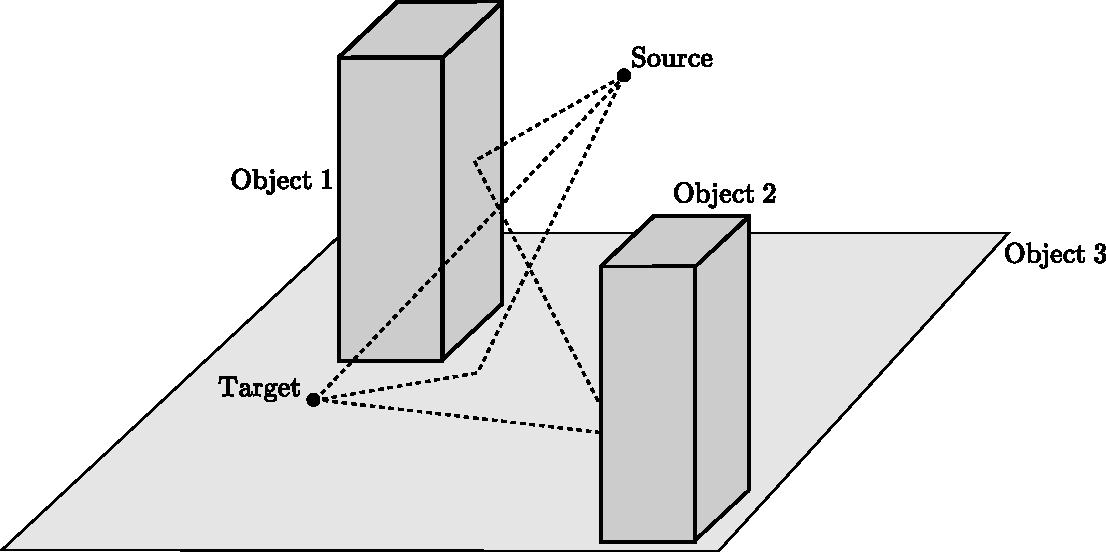
\includegraphics[width=0.7\linewidth]{figures/path-solver-scene.pdf}
    \caption{The path solver constructs propagation paths that connect a source and a target in a scene.\label{fig:paths}}
\end{figure}

A path solver aims to determine a set of paths that connect two endpoints in a scene, as illustrated in Figure~\ref{fig:paths}.
From this set of paths, a time- or frequency-domain \gls{CIR} can be computed.
The path solver leverages \gls{SBR} to efficiently compute paths in a scene.
\Gls{SBR} operates as follows:
First, rays\footnote{The processing of the rays is parallelized for accelerated computation.} are traced from the source into directions specified by a lattice on the unit sphere (see Section~\ref{sec:path-solver-fibonacci}).
Then, an \gls{SBR} loop iteratively tests the intersection of the rays with the scene geometry.
At every intersection, an interaction type is selected from $\Ic$, and a new ray is spawned according to the selected interaction type.
The method for choosing interaction types is detailed in Section~\ref{sec:path-solver-interaction-sampling}.
The loop terminates when no more rays remain \emph{active}, meaning they have either bounced out of the scene, reached a predefined maximum number of bounces, or satisfied another termination criterion.
Notably, at each interaction of a ray with a surface in the scene, only one scattered ray is spawned, as spawning multiple rays would result in an exponential increase in the number of rays, quickly overwhelming the available computational resources.

When a diffuse reflection occurs during the \gls{SBR} loop, the solver checks whether there is a \gls{LoS} to the target, meaning that the ray segment from the interaction point to the target point is not occluded. If such a connection exists, the path is deemed valid and is returned by the solver. This process is known as \emph{next-event estimation}. Subsequently, a new ray is spawned in a random direction within the hemisphere defined by the surface normal of the primitive involved. This new ray may lead to the discovery of additional paths.
Next-event estimation is only possible for diffuse reflections that scatter energy into all directions.
For specular reflection and refraction, only a single ray is spawned in the only possible direction.
Consequently, the probability of finding paths connecting the source to the target that end with a specular reflection or refraction by \gls{SBR} is effectively zero, as depicted in Figure~\ref{fig:sbr-specular-diffuse}.
This is because hitting a specific point (the target) with a specular reflection or refraction requires perfect alignment of the incident ray, which has zero probability in continuous space.
Likewise, for diffraction, the probability that the target is on the surface of the Keller cone is zero, as shown in Figure~\ref{fig:sbr-diffraction}.
When diffraction occurs, a single ray is spawned in a random direction along the Keller cone to continue the sample.
Paths ending with a specular suffix can therefore not be determined solely by \gls{SBR}.
In particular, specular chains cannot be computed by \gls{SBR}.
Since specular chains typically carry a significant amount of the transported energy, \gls{SBR} alone is insufficient for computing \glspl{CIR}.

\begin{figure}[ht!]
    \centering
    \begin{subfigure}[b]{0.45\textwidth}
        \centering
        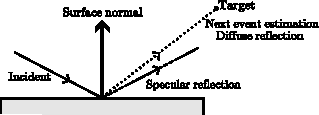
\includegraphics[width=\textwidth]{figures/path-solver-sbr-spec-diff.pdf}
        \subcaption{\label{fig:sbr-specular-diffuse}}
    \end{subfigure}
    \hspace{1em}
    \begin{subfigure}[b]{0.45\textwidth}
        \centering
        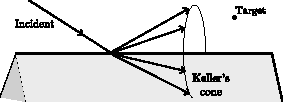
\includegraphics[width=\textwidth]{figures/path-solver-sbr-diffr.pdf}
        \subcaption{\label{fig:sbr-diffraction}}
    \end{subfigure}
    \caption{(a) When a diffuse reflection occurs, next event estimation tests whether the \gls{LoS} between the intersection point and the target is occluded (represented by the dotted line). This process is not applicable for specular reflection (represented by the dashed line) and refraction, as only one single direction for the scattered ray is valid. (b) Similarly, for diffraction, the probability that the target is on the surface of the Keller cone is zero, and a single ray is spawned in a random direction along the Keller cone to continue the sample. Shown in 2D for clarity.}
\end{figure}

To compute paths ending with a specular suffix, including specular chains, the path solver uses an \emph{image method}-based algorithm.
However, a brute-force implementation of the image method that would test all possible combinations of primitives and wedges that constitute the scene is prohibitive even for moderately large scenes.
Therefore, the path solver uses \gls{SBR} as a heuristic to find \emph{path candidates}.
A path candidate consists of a sequence of primitives or wedges and interaction types ending with a specular reflection, refraction, or diffraction. As the path vertices determined during the \gls{SBR} do not form a path that connects to the target, the image method is used to adjust the vertex locations to establish the connection.
Intuitively, \gls{SBR} pre-selects path candidates in the vicinity of the transmitter and receiver for the image method to compute corresponding valid paths to be returned by the solver.
These steps of the \SRT{} path solver are depicted in Figure~\ref{fig:path-solver-archi}.
Notably, only path candidates ending with a specular suffix (including specular chains) require further processing by the image method algorithm.
Finally, for each valid path identified, the path solver computes the corresponding channel coefficients and propagation delays that characterize the \gls{EM} wave propagation along that path.

Alternative methods for identifying paths that include specular chains or specular suffixes may involve detection spheres centered at the targets to capture paths ending with a specular suffix, and/or extending the direction of specular reflection (or refraction) to a lobe around the specular, refracted, or diffracted direction. Such methods only approximate the path vertex locations and the directions of the scattered rays, yielding inaccurate path coefficients and resulting in incorrect \glspl{CIR}.

\begin{figure}[ht!]
    \centering
    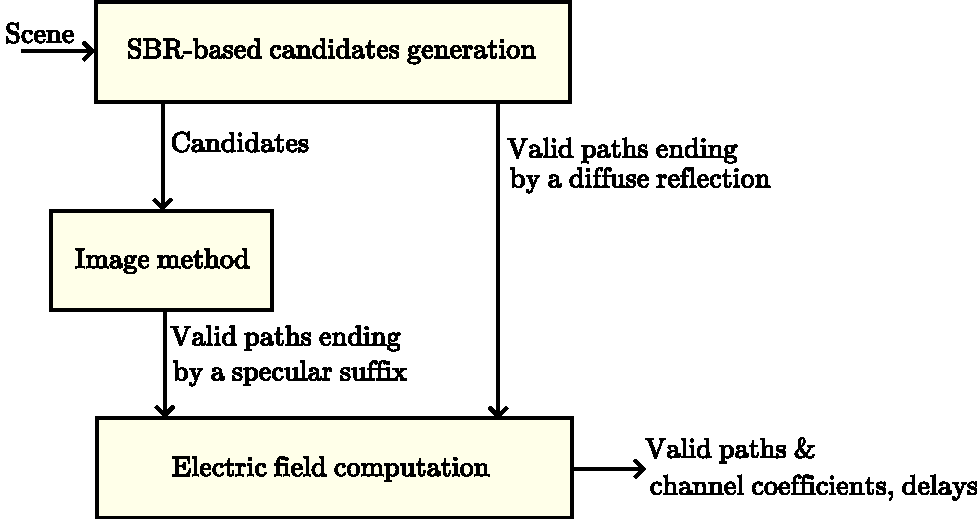
\includegraphics[width=0.65\textwidth]{figures/path-solver-arch.pdf}
    \caption{Main steps of the \SRT{} path solver.\label{fig:path-solver-archi}}
\end{figure}

The remainder of this section follows the architecture of the path solver shown in Figure~\ref{fig:path-solver-archi}.
First, Section~\ref{sec:path-solver-sbr} presents the \gls{SBR}-based candidate generator.
Section~\ref{sec:path-solver-im} then describes the image method-based algorithm that processes candidates to find valid paths with specular suffixes.
Section~\ref{sec:path-solver-em} details how the solver computes the complex-valued channel coefficients and propagation delays, which characterize the radio channel.
Finally, Section~\ref{sec:path-solver-limitations} discusses current limitations and potential improvements of the path solver.

\subsection{Generating Candidates by Shooting and Bouncing of Rays (SBR)}
\label{sec:path-solver-sbr}

\begin{figure}[ht!]
    \centering
    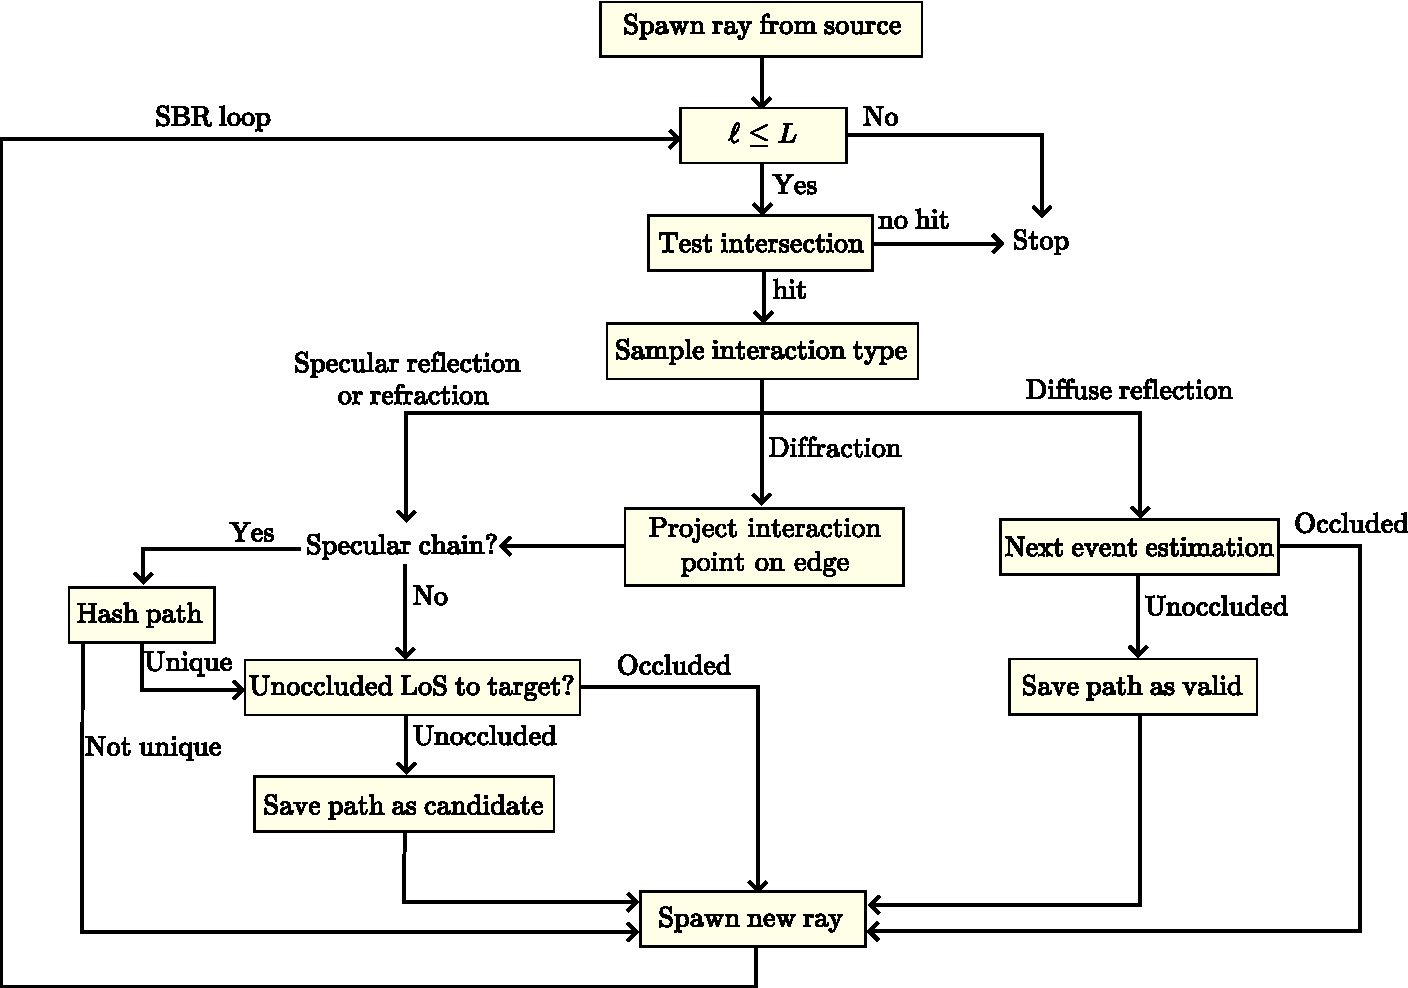
\includegraphics[width=0.95\textwidth]{figures/path-solver-sbr.pdf}
    \caption{Algorithm for one sample as implemented in the \gls{SBR}-based candidate generator. In practice, many samples are processed in parallel.}
    \label{fig:path-solver-sbr}
\end{figure}

The candidate generator utilizes the \gls{SBR}-based method as illustrated in Figure~\ref{fig:path-solver-sbr}.
We first provide an overview of the \gls{SBR} procedure, followed by a detailed explanation.
We consider a scene with a single source located at $\sv \in \RR^3$ and $N_T$ targets at $\tv_k \in \RR^3$, where $k = 1, \dots, N_T$.
Although the path solver built into \SRT{} can handle multiple sources, we focus on a single source for the sake of clarity. The process is identical for all sources.
The paths traced by the candidate generator during the \gls{SBR} procedure are referred to as \emph{samples} in this section to avoid confusion with the valid paths returned to the user and the candidate paths forwarded to the image method-based algorithm.
A sample therefore consists of a sequence of rays connected end-to-end, traced by the candidate generator.
As we will see, a single sample can result in multiple valid or candidate paths, as illustrated in Figure~\ref{fig:path-solver-sbr-samples}.

\begin{figure}[ht!]
    \centering
    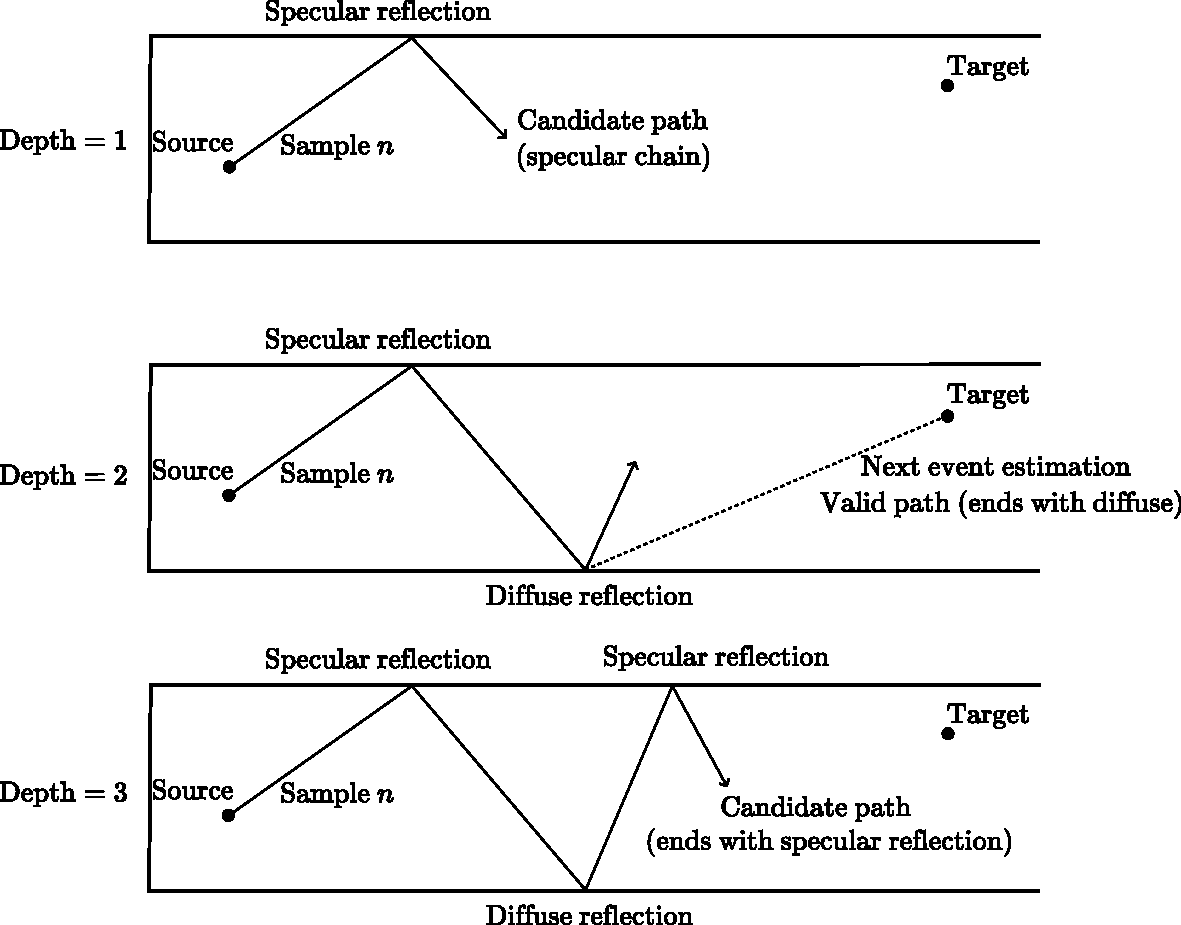
\includegraphics[width=0.75\textwidth]{figures/path-solver-sbr-sample.pdf}
    \caption{\gls{SBR} procedure for a single sample $n$ at depths 1, 2, and 3. At each interaction (i.e. iteration of the \gls{SBR} loop), the sample may result in a candidate or valid path, and a new ray is spawned from the current interaction point to prolong the sample path. Shown in 2D for clarity.\label{fig:path-solver-sbr-samples}}
\end{figure}

The \gls{SBR} procedure begins by spawning a user-specified number of rays, denoted by $N_S$, from the source $\sv$ in directions $\widehat{\kv}_n^{(0)}$ on a Fibonacci lattice, where $n = 1, \dots, N_S$.
Each ray starts a sample that is traced by the candidate generator.
Details on the implemented Fibonacci lattice can be found in Section~\ref{sec:path-solver-fibonacci}.
The \gls{SBR} loop then iterates until either all samples bounce out of the scene or reach a user-specified maximum number of bounces, denoted as the \emph{maximum depth} $L$.
We denote the depth of the samples by $\ell = 0, \dots, L$.
The first step of the \gls{SBR} loop involves testing the intersection of the samples with the scene geometry.
If a sample does not intersect any object, it has bounced out of the scene, and is deactivated.
When a sample $n$ with depth $\ell$ intersects the scene, we denote by $\vv_n^{(\ell)} \in \RR^3$ the intersection point, by $\widehat{\nv}_n^{(\ell)} \in \RR^3~\LB \norm{\widehat{\nv}_n^{(\ell)}} = 1 \RB$ the surface normal at the intersection point oriented towards the half-space containing the incident field, by $o_n^{(\ell)} \in \NN_0$ the index of the intersected object, and by $m_n^{(\ell)} \in \NN_0$ the index of the specific intersected primitive within that object.
The interaction type, denoted by $\chi_n^{(\ell)}$, is then sampled from $\Ic$, determining how the sample will continue to propagate.
Details on the sampling of the interaction type are provided in Section~\ref{sec:path-solver-interaction-sampling}.
The rest of the loop depends on the sampled interaction type.

\paragraph{Diffuse Reflection}
As previously indicated, diffuse reflection is assumed to scatter energy in all directions of the half-space containing the incident field, which enables next event estimation.
Therefore, if a diffuse reflection is sampled (i.e. $\chi_n^{(\ell)} = \Sc$), the \gls{LoS} between the intersection point and each target $\tv_1, \cdots, \tv_{N_T}$ is tested.
For each target $\tv_k$ with an unobstructed \gls{LoS} to the intersection point, a path connecting the source to the target
\begin{equation}
    \label{eq:path-solver-sample-path}
    p_n^{(\ell)} = \left(\sv, \vv_n^{(1)}, \cdots, \vv_n^{(\ell)}, \tv_k\right)
\end{equation}
is recorded as a valid path to be returned to the user.
Finally, a new ray is spawned to continue the sample path, with its direction selected uniformly at random from the hemisphere defined by $\widehat{\nv}_n^{(\ell)}$, i.e. $\widehat{\kv}_{n}^{(\ell)} \sim \Uc_{2\pi}(\widehat{\nv}_n^{(\ell)})$, where $\Uc_{2\pi}(\widehat{\nv}_n^{(\ell)})$ represents the uniform distribution on the hemisphere.

\paragraph{Specular Reflection and Refraction}
When a specular reflection or refraction is sampled (i.e. $\chi_n^{(\ell)} = \Rc$ or $\chi_n^{(\ell)} = \Tc$), the path~\eqref{eq:path-solver-sample-path} is a valid path for target $\tv_k$, where $k \in \left\{1, \dots, N_T\right\}$, only if
\begin{equation}
    \label{eq:path-solver-spec-cond}
    \frac{\tv_k - \vv_n^{(\ell)}}{\norm{\tv_k - \vv_n^{(\ell)}}} = \widehat{\kv}_n^{(\ell)},
\end{equation}
where
\begin{equation}
    \label{eq:path-solver-scatter-dir}
    \widehat{\kv}_n^{(\ell)} =
    \begin{cases}
        \frac{\widehat{\kv}_n^{(\ell-1)} - 2 \LB\LB\widehat{\kv}_n^{(\ell-1)}\RB\tp \widehat{\nv}_n^{(\ell)}\RB \widehat{\nv}_n^{(\ell)}}{\norm{\widehat{\kv}_n^{(\ell-1)} - 2 \LB\LB\widehat{\kv}_n^{(\ell-1)}\RB\tp \widehat{\nv}_n^{(\ell)}\RB \widehat{\nv}_n^{(\ell)}}} & \text{if } \chi_n^{(\ell)} = \Rc  \\
        \widehat{\kv}_n^{(\ell-1)} & \text{if } \chi_n^{(\ell)} = \Tc
    \end{cases}
\end{equation}
and where $\uv\tp$ denotes the transpose of $\uv$.
Since targets are modeled as points, condition~\eqref{eq:path-solver-spec-cond} effectively occurs with zero probability, and, consequently, the path~\eqref{eq:path-solver-sample-path} is not a valid path.
However, the specular suffix $p_n^{(\ell_d:)}$, where $\ell_d$ is defined as in~\eqref{eq:essential-concepts-ell_d}, can be further processed to determine vertices $\left(\widetilde{\vv}_n^{(\ell_d+1)}, \cdots, \widetilde{\vv}_n^{(\ell)}\right)$ such that
\begin{equation}
    \label{eq:path-solver-complete-cand}
    \widetilde{p}_n^{(\ell)} = \LB\sv, \vv_n^{(1)}, \cdots,
    \underbrace{\widetilde{\vv}_n^{(\ell_d+1)}, \cdots, \widetilde{\vv}_n^{(\ell)}, \tv_k}_{\text{Processed specular suffix}}\RB
\end{equation}
is a valid path, as illustrated in Figure~\ref{fig:path-solver-sbr-cand-im}.
This additional processing is performed using the image method in the algorithm described in Section~\ref{sec:path-solver-im}.

\begin{figure}[ht!]
    \centering
    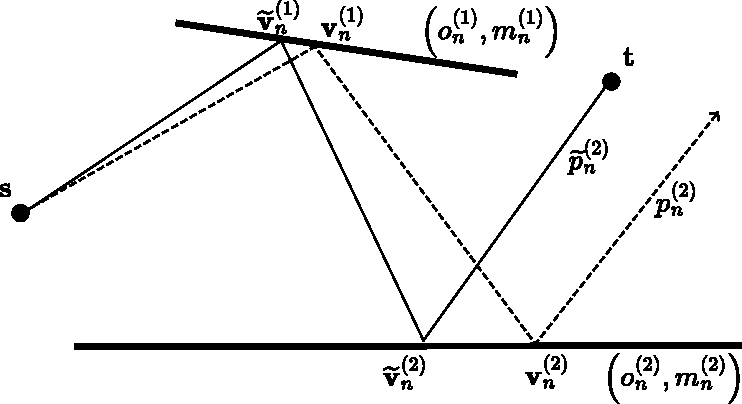
\includegraphics[width=0.55\textwidth]{figures/path-solver-sbr-cand-im.pdf}
    \caption{Processing a candidate specular chain of depth $\ell = 2$ ($p_n^{(2)}$, dashed line) to produce a valid path ($\widetilde{p}_n^{(2)}$, solid line). The same process applies to specular suffixes. Shown in 2D for clarity.\label{fig:path-solver-sbr-cand-im}}
\end{figure}

Importantly, for a sequence of primitives and interaction types
\begin{equation}
    \label{eq:path-solver-cand}
    \LB \vv_n^{(\ell_d)}, \LB o_n^{(\ell_d+1)}, m_n^{(\ell_d+1)}, \chi_n^{(\ell_d+1)} \RB, \cdots, \LB o_n^{(\ell)}, m_n^{(\ell)}, \chi_n^{(\ell)} \RB, \tv_i\RB
\end{equation}
where $\vv_n^{(0)} = \sv$, there exists \emph{at most a single} set of vertices $\widetilde{\vv}_n^{(\ell_d+1)},\cdots,\widetilde{\vv}_n^{(\ell)}$ such that $\widetilde{p}_n^{(\ell)}$ is a valid path.
Consequently, if $\ell_d = 0$, i.e. $p_n^{(\ell)}$ is a specular chain, then further processing by the image method of multiple identical candidates~\eqref{eq:path-solver-cand} would result in multiple identical valid paths, which would lead to erroneous \glspl{CIR}.
Therefore, if the sample $p_n^{(\ell)}$ is a specular chain, a hashing-based de-duplication mechanism, detailed in Section~\ref{sec:path-solver-hashing},  ensures that specular chain candidates are only evaluated once.
Notably, the path hashing mechanism discards redundant candidates ``on-the-fly'', significantly reducing memory and compute requirements.
However, when $\ell_d > 0$, then $\vv_n^{(\ell_d)}$ corresponds to a diffuse reflection point that is the result of a randomly sampled ray direction (either at the source or the last previous diffuse reflection point).
Since the probability of two different paths having identical randomly sampled diffuse reflection points is effectively zero, path uniqueness is guaranteed in these cases without requiring the de-duplication mechanism.

As shown in Figure~\ref{fig:path-solver-sbr}, a \gls{LoS} occlusion test to the target is used as a heuristic to discard path candidates that have little chance of resulting in a valid path after processing by the image method-based algorithm.
Finally, a new ray is traced into the direction~\eqref{eq:path-solver-scatter-dir} to continue the sample path.

\paragraph{Diffraction}
\begin{figure}[ht!]
    \centering
    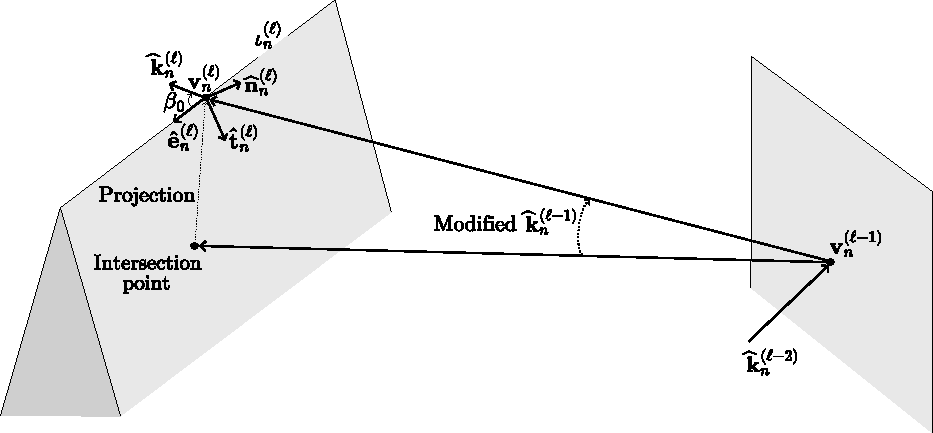
\includegraphics[width=0.75\textwidth]{figures/path-solver-proj-diffr.pdf}
    \caption{Diffracting edges are identified by projecting the intersection point onto the edges of the intersected primitive.\label{fig:path-solver-diffr-proj}}
\end{figure}
When tracing rays, the probability that a ray exactly intersects the edge of a wedge is zero.
Therefore, when a ray intersects a primitive and diffraction is sampled (i.e., $\chi_n^{(\ell)} = \Dc$), the intersection point between the ray $\left( \vv_n^{(\ell-1)}, \widehat{\kv}_n^{(\ell-1)}\right)$ and the primitive $\left(o_n^{(\ell)}, m_n^{(\ell)}\right)$ is projected onto one of the primitive's edges, yielding the vertex $\vv_n^{(\ell)}$, as illustrated in Figure~\ref{fig:path-solver-diffr-proj}.
The index of the edge onto which the intersection point is projected is denoted by $\iota^{(\ell)}_n$.

The path~\eqref{eq:path-solver-sample-path} is a valid path to a target $\tv_k$ (with $k \in \{1, \dots, N_T\}$) only if there exists an angle $\phi \in [0, n\pi]$, where $n\pi$ is the exterior angle of the wedge, such that
\begin{equation}
    \label{eq:path-solver-diffr-cond}
    \frac{\tv_k - \vv_n^{(\ell)}}{\norm{\tv_k - \vv_n^{(\ell)}}} = \widehat{\kv}_n^{(\ell)},
\end{equation}
with the diffraction direction given by
\begin{equation}
    \label{eq:path-solver-k_diffr}
    \widehat{\kv}_n^{(\ell)} = \sin{\left(\beta_0\right)}\cos{\phi} \widehat{\mathbf{t}}_n^{(\ell)}
                               + \sin{\left(\beta_0\right)}\sin{\phi} \widehat{\nv}_n^{(\ell)}
                               + \cos{\left(\beta_0\right)} \widehat{\mathbf{e}}_n^{(\ell)},
\end{equation}
where $\beta_0$ is the angle between the incident ray direction $\widehat{\kv}_n^{(\ell-1)}$ and the wedge vector $\widehat{\mathbf{e}}_n^{(\ell)}$, and $\left(\widehat{\mathbf{t}}_n^{(\ell)}, \widehat{\nv}_n^{(\ell)}, \widehat{\mathbf{e}}_n^{(\ell)}\right)$ is an orthonormal basis such that $\widehat{\mathbf{t}}_n^{(\ell)} = \widehat{\nv}_n^{(\ell)} \times \widehat{\mathbf{e}}_n^{(\ell)}$ (see Figure~\ref{fig:path-solver-diffr-proj}).
Note that $\widehat{\tv}_n^{(\ell)}$ is tangent to the wedge face.
In~\eqref{eq:path-solver-k_diffr}, ensuring that the angle between the diffracted ray and the edge, denoted by $\beta_0$, matches the angle between the incident ray and the edge, places the ray on the Keller cone.
As with specular reflection and refraction, since targets are modeled as points, condition~\eqref{eq:path-solver-diffr-cond} is satisfied with zero probability for all $\phi \in [0, n\pi]$, rendering the sampled path invalid.
Therefore, candidate paths ending with a diffraction are further refined using the image method-based algorithm described in Section~\ref{sec:path-solver-im}, just as for paths ending with specular reflection or refraction.
As shown in Figure~\ref{fig:path-solver-sbr}, the processing of diffraction thus follows the same steps as for specular reflection and refraction: a hashing-based de-duplication mechanism ensures uniqueness of specular chains, and an occlusion test to the target is used as a heuristic to eliminate candidates unlikely to produce valid paths after refinement with the image method.
Finally, a new ray is traced in the direction~\eqref{eq:path-solver-k_diffr} to continue the sample path, with $\phi$ sampled uniformly from $[0, n\pi]$.

As illustrated in Figure~\ref{fig:path-solver-diffr-proj}, projecting the intersection point onto an edge alters the scattered ray direction $\widehat{\kv}_n^{(\ell-1)}$ departing from $\vv_n^{(\ell-1)}$.
This modification invalidates any preceding specular reflections or refractions, meaning that path segments that are not suffixes would require refinement if a diffraction is followed by a diffuse reflection.
To avoid significantly increased computational complexity from refining non-suffix path segments, the path solver prohibits sampling paths that contain both diffraction and diffuse reflection.
Such paths typically contribute negligibly to the total transported energy and therefore have little impact on the accuracy of the \glspl{CIR}.
Moreover, \SRT{} currently supports only first-order diffraction, meaning that paths may contain at most one diffraction event.

The candidate generator depicted in Figure~\ref{fig:path-solver-sbr} thus yields a set of valid paths connecting the source to all targets that do not require further processing (except for the computation of the corresponding path coefficients and delays) and end with a diffuse reflection.
Additionally, it produces a set of candidate paths ending with specular suffixes, which require further processing to be either discarded or refined into valid paths.

\begin{figure}[htbp]
    \centering
    % First subfigure
    \begin{subfigure}[b]{0.3\textwidth}
        \centering
        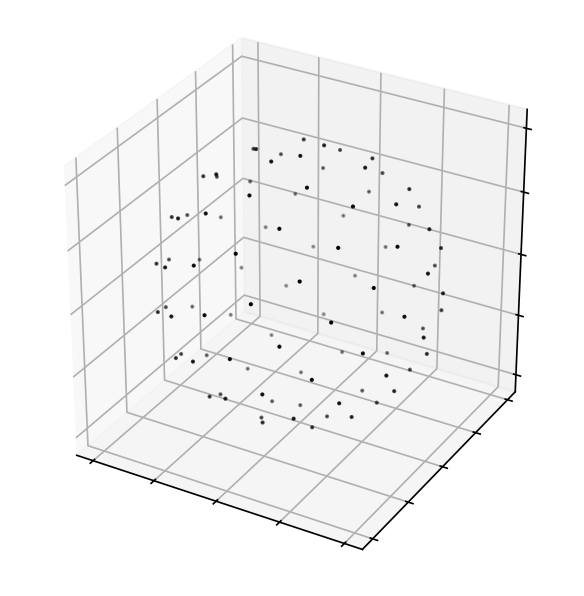
\includegraphics[width=\textwidth]{figures/path-solver-fibo-100.png}
        \caption{100 points.}
    \end{subfigure}
    \hfill
    % Second subfigure
    \begin{subfigure}[b]{0.3\textwidth}
        \centering
        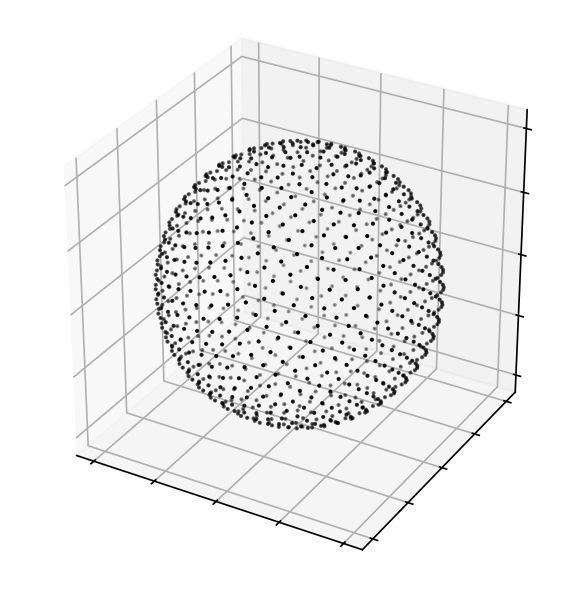
\includegraphics[width=\textwidth]{figures/path-solver-fibo-1000.png}
        \caption{1000 points.}
    \end{subfigure}
    \hfill
    % Third subfigure
    \begin{subfigure}[b]{0.3\textwidth}
        \centering
        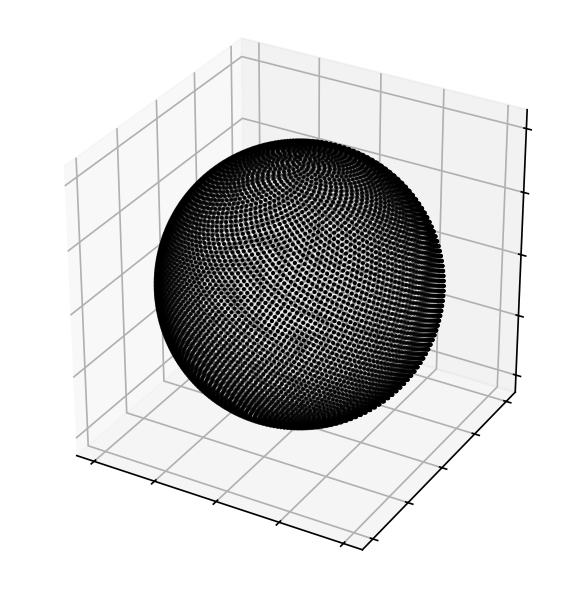
\includegraphics[width=\textwidth]{figures/path-solver-fibo-10000.png}
        \caption{10000 points.}
        \end{subfigure}
    \caption{Spherical Fibonacci lattice.\label{fig:path-solver-fibonacci}}
\end{figure}

\subsubsection{Sampling Initial Ray Directions}
\label{sec:path-solver-fibonacci}

The \gls{SBR} procedure starts by spawning rays from the source with directions obtained from a spherical Fibonacci lattice with $N_S$ points, which is defined as follows:
\begin{equation}
    \widehat{\kv}_n^{(0)} =
    \begin{bmatrix}
        \sin{\theta_n}\cos{\phi_n}\\
        \sin{\theta_n}\sin{\phi_n}\\
        \cos{\theta_n}
    \end{bmatrix}
\end{equation}
where
\begin{eqnarray*}
    \theta_n &= & \arccos{\frac{2n}{N_S}}\\
    \phi_n &= & 2\pi\frac{n}{\varphi}
\end{eqnarray*}
and $-\left\lfloor\frac{N_S}{2}\right\rfloor \leq n \leq \left\lceil \frac{N_S}{2} \right\rceil - 1$, $\varphi = \frac{1 + \sqrt{5}}{2}$ is the golden ratio, and $\left\lfloor \cdot \right\rfloor$ and $\left\lceil \cdot \right\rceil$ the floor and ceiling function, respectively.
Note that when defining the Fibonacci lattice, the index $n$ takes values in the range $-\left\lfloor\frac{N_S}{2}\right\rfloor, \dots, \left\lceil \frac{N_S}{2} \right\rceil - 1$ instead of the usual $1,\dots,N_S$.
Sampling rays from the Fibonacci lattice results in ray tubes sharing approximately the same opening angle $\frac{4\pi}{N_S}$.

The Fibonacci lattice was selected for its simple construction and its benefits over other lattices for numerical integration~\cite{gonzalez2010measurement,hannay2004fibonacci}.
Figure~\ref{fig:path-solver-fibonacci} shows the spherical Fibonacci lattice with 100, 1000, and 10000 points.
The \SRT{} path solver uses $10^6$ points as the default value for $N_S$, and higher values will ensure that more valid paths are found.

\subsubsection{Sampling Interaction Types}
\label{sec:path-solver-interaction-sampling}

Within the \gls{SBR} loop, when a ray intersects the scene geometry, the algorithm generates at most one scattered ray. This constraint is necessary because generating multiple rays at each intersection, such as both reflected and refracted rays, would lead to an exponential increase in computational complexity and memory usage with the depth of the path. Instead, a single interaction type is randomly chosen based on a distribution:
\begin{equation}
    \label{eq:path-solver-int-dist}
\Qc  = \LP q\LB\Rc\RB, q\LB\Sc\RB, q\LB\Tc\RB, q\LB\Dc\RB \RP,\qquad \text{where } q\LB\Rc\RB + q\LB\Sc\RB + q\LB\Tc\RB + q\LB\Dc\RB = 1 \text{ and } q\LB\cdot\RB \geq 0.
\end{equation}
Here, $q \LB \chi \RB$ represents the probability of selecting the interaction type $\chi \in \Ic$. Importantly, the choice of distribution $\Qc$ does not affect the calculation of the paths' electric fields, which are solely dependent on the propagation environment. However, the choice of distribution $\Qc$ significantly impacts the \emph{sample efficiency} of the ray tracer, which affects the number of samples $N_S$ needed to compute paths that connect a source to a target and capture the majority of the transported energy.
Sampling only one interaction type per intersection may appear limiting, but this is offset by the large number of samples generated from each source. In most scenarios, a high sample count allows identifying all significant paths.

For each sample $n$ at depth $\ell$, the interaction type is sampled independently for every interaction along every path.
For specular reflection, diffuse reflection, and refraction, the probability of selecting each interaction type is proportional to the squared amplitudes of the corresponding reflection and refraction coefficients.
Diffraction, on the other hand, is sampled using a fixed probability $q\LB\Dc\RB \in [0, 1]$.
This choice is motivated by the fact that diffraction typically carries much less energy compared to reflection and refraction, which would result in very low probabilities for sampling diffraction if its probability were also based on the diffraction coefficients.
The resulting distribution for the interaction types is:
\begin{equation}
    \label{eq:path-solver-used-dist-event}
    \begin{aligned}
        q\LB\Rc\RB &= \left(1 - q\LB\Dc\RB\right)R^2\frac{\abs{r_{\perp}}^2 + \abs{r_{\parallel}}^2}{\abs{r_{\perp}}^2 + \abs{r_{\parallel}}^2 + \abs{t_{\perp}}^2 + \abs{t_{\parallel}}^2}\\
        q\LB\Sc\RB &= \left(1 - q\LB\Dc\RB\right)S^2\frac{\abs{r_{\perp}}^2 + \abs{r_{\parallel}}^2}{\abs{r_{\perp}}^2 + \abs{r_{\parallel}}^2 + \abs{t_{\perp}}^2 + \abs{t_{\parallel}}^2}\\
        q\LB\Tc\RB &= \left(1 - q\LB\Dc\RB\right)\frac{\abs{t_{\perp}}^2 + \abs{t_{\parallel}}^2}{\abs{r_{\perp}}^2 + \abs{r_{\parallel}}^2 + \abs{t_{\perp}}^2 + \abs{t_{\parallel}}^2}\\
        q\LB\Dc\RB &\in [0, 1]
    \end{aligned}
\end{equation}
In \SRT{}, $q\LB \Dc \RB$ is set to $0.2$.
Here, $r_{\perp}$, $r_{\parallel}$, $t_{\perp}$, and $t_{\parallel}$ are the Fresnel coefficients~\eqref{eq:fresnel_slab}, $S$ is the scattering coefficient (see Section~\ref{sec:primer-em-diffuse}), and $R$ is the reflection reduction factor~\eqref{eq:R}. This approach ensures that interaction types responsible for scattering more energy are sampled more frequently—-a technique known as \emph{importance sampling}~\cite{Kloek1978, Wikipedia_Importance_Sampling}.
This is similar to importance sampling techniques for light transport paths commonly used in computer graphics.
A brief overview of importance sampling in the context of ray tracing for the simulation of radio wave propagation is provided in Appendix~\ref{sec:importance-sampling}.

\begin{figure}[t]
    \centering
    \begin{subfigure}[b]{0.48\textwidth}
        \centering
        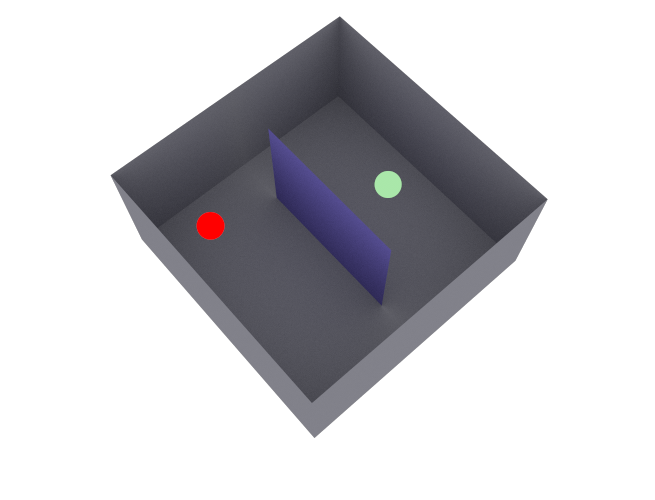
\includegraphics[width=\textwidth]{figures/importance-sampling-uniform-heuristic-scene.png}
        \caption{Scene used for the comparison.}
        \label{fig:path-solver-sampling-scene}
    \end{subfigure}
    \hfill
    \begin{subfigure}[b]{0.48\textwidth}
        \centering
        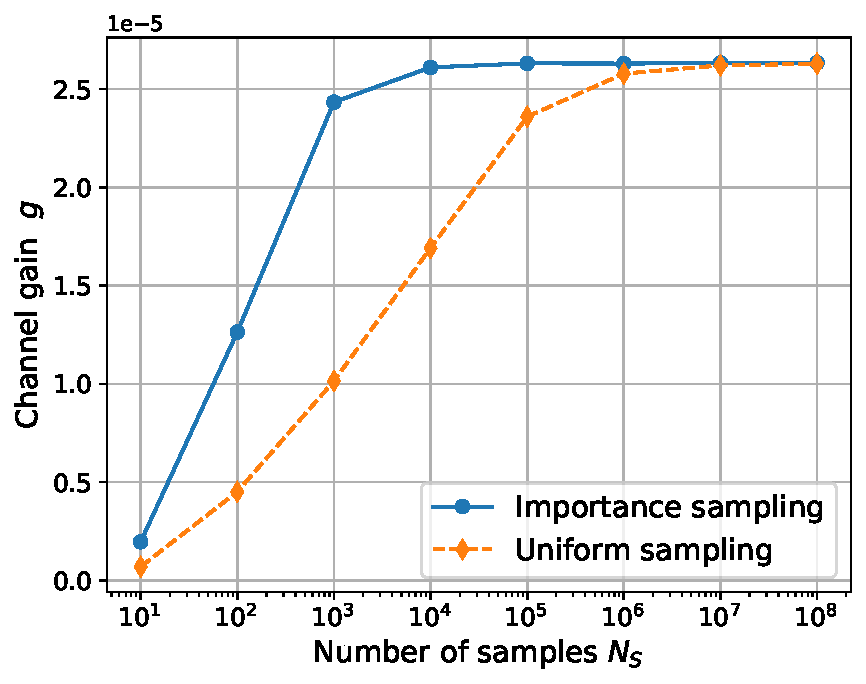
\includegraphics[width=\textwidth]{figures/importance-sampling-uniform-heuristic.pdf}
        \caption{Channel gain at the target.}
        \label{fig:path-solver-sampling-importance}
    \end{subfigure}
    \caption{Comparison of sampling strategies for interaction types. The scene consists of a closed metallic box containing a glass screen, with a source (red ball) and target (green ball) on opposite sides. The box is shown open to visualize the interior. Importance sampling achieves faster convergence of the channel gain compared to uniform sampling.}
    \label{fig:path-solver-sampling}
\end{figure}

To illustrate the importance of optimized sampling strategies, we compare uniform sampling, where specular reflection, diffuse reflection, and refraction are selected with equal probability, to importance sampling using the scene shown in Figure~\ref{fig:path-solver-sampling-scene}. The scene consists of a metallic box containing a glass screen, with a source and target positioned on opposite sides.
Diffuse reflection, specular reflection, refraction, and diffraction are enabled, and the maximum depth $L$ is set to $5$.
As shown in Figure~\ref{fig:path-solver-sampling-importance}, using importance sampling leads to better sample efficiency when compared to uniform sampling, as convergence requires approximately $100\times$ fewer samples to capture most of the received energy. This demonstrates the benefit of selecting interactions according to the material properties of the scatterers.

\subsubsection{Specular Chain Candidates Deduplication}
\label{sec:path-solver-hashing}

As mentioned in Section~\ref{sec:path-solver-sbr} and Figure~\ref{fig:path-solver-sbr}, to avoid storing multiple identical specular chain candidates, a path hashing method is used to discard duplicates of previously found candidates ``on-the-fly''.
A specular chain candidate is defined by a sequence of interactions with the scene, each characterized by the intersected object $o_n^{(\ell)} \in \NN_0$, the corresponding intersected primitive $m_n^{(\ell)} \in \NN_0$, the diffracted edge $\iota_n^{(\ell)} \in \{0, 1, 2\}$ (if $\chi_n^{(\ell)} = \Dc$), and the interaction type $\chi_n^{(\ell)} \in \LP \Rc, \Tc, \Dc \RP$ with $\ell_d = 0$, i.e.
\begin{equation}
    c^{(\ell)}_n = \LB \sv, \LB o_n^{(1)}, m_n^{(1)}, \iota_n^{(1)}, \chi_n^{(1)} \RB, \cdots, \LB o_n^{(\ell)}, m_n^{(\ell)}, \iota_n^{(\ell)}, \chi_n^{(\ell)} \RB \RB.
\end{equation}
For specular chain candidates, we do not need to store the path vertices. If the candidate leads to a valid path, these vertices will be computed. Invalid candidates are discarded.

\begin{figure}[ht!]
    \centering
    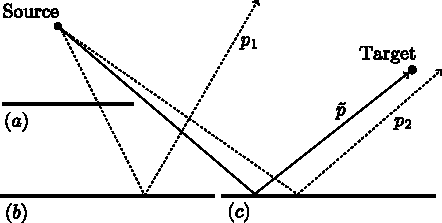
\includegraphics[width=0.51\textwidth]{figures/path-solver-hashing-coplanar.pdf}
    \caption{Two candidate paths, $p_1$ and $p_2$, which differ by being reflected by different coplanar primitives and by encountering a refraction (in $p_1$ only), yield the same path $\widetilde{p}$ once refined by the image method. Shown in 2D for clarity.\label{fig:path-solver-hashing-coplanar}}
\end{figure}

The hashing process guarantees that each specular chain candidate uniquely represents the geometry of a path after refinement with the image method (see Section~\ref{sec:path-solver-im}).
This is achieved by computing a hash value that uniquely identify the sequence of primitives constituting the path.
Importantly, primitives that are coplanar (i.e., lie in the same plane) are treated as equivalent during hashing.
This is because the image method assumes all reflection surfaces extend infinitely, making the exact in-plane position of a primitive irrelevant to the path geometry.
Furthermore, refraction can be omitted from the hashing procedure since it does not change the ray direction and therefore does not alter the geometry of the path, as refraction is modeled without angular deflection.
Figure~\ref{fig:path-solver-hashing-coplanar} illustrates this concept: two candidate paths, $p_1$ and $p_2$, yield to the same refined path $\widetilde{p}$, and thus they should share the same hash value.
This holds even though only one candidate is refracted by primitive $(a)$, and both are reflected by different but coplanar primitives $(b)$ and $(c)$, respectively.

\begin{algorithm}
    \begin{center}
    \begin{algorithmic}[1]
        \State $\texttt{hash}_n^{(0)} \gets 0$
        \State $\ell \gets 1$
        \While{\text{<Stop condition>}} \Comment{\gls{SBR} loop}
            \State $\cdots$
            \State $\texttt{inter\_hash}_{n}^{(\ell)} \gets \Call{hash\_intersection}{o_n^{(\ell)}, m_n^{(\ell)}, \iota_n^{(\ell)}, \chi_n^{(\ell)}}$
            \State $\texttt{hash}_n^{(\ell)} \gets \Call{hash\_update}{\texttt{hash}_n^{(\ell-1)}, \texttt{inter\_hash}_{n}^{(\ell)}}$
            \State $\cdots$
            \State $\ell \gets \ell + 1$
        \EndWhile
        \State
        \Procedure{hash\_intersection}{$o, m, \iota, \chi$}
            \If{$\chi = \Rc$}
                \Return $\Call{hash\_plane}{o,m}$
            \ElsIf{$\chi = \Dc$}
                \Return $\Call{hash\_edge}{o,m, \iota}$
            \EndIf
        \EndProcedure
        \State
        \Procedure{hash\_plane}{$o, m$}
            \State $\nv \gets \Call{get\_normal}{o, m}$ \Comment{Read the primitive normal}
            \State $\pv \gets \Call{get\_vertex}{o, m}$ \Comment{Read a primitive vertex}
            \State $d \gets \nv\tp \pv$ \Comment{Offset of the plane to the origin}
            \State $h \gets \Call{FNV1a}{\texttt{Q}(\nv_x), \texttt{H}}$
            \State $h \gets \Call{FNV1a}{\texttt{Q}(\nv_y), h}$
            \State $h \gets \Call{FNV1a}{\texttt{Q}(\nv_z), h}$
            \State $h \gets \Call{FNV1a}{\texttt{Q}(d), h}$
            \State \Return $h$
        \EndProcedure
        \State
        \Procedure{hash\_edge}{$o, m, \iota$}
            \State $\pv_1, \pv_2 \gets \Call{get\_endpoints}{o, m, \iota}$ \Comment{Read the edge endpoints}
            \State $h \gets \Call{FNV1a}{\texttt{Q}(\pv_{1,x}), \texttt{H}}$
            \State $h \gets \Call{FNV1a}{\texttt{Q}(\pv_{1,y}), h}$
            \State $h \gets \Call{FNV1a}{\texttt{Q}(\pv_{1,z}), h}$
            \State $h \gets \Call{FNV1a}{\texttt{Q}(\pv_{2,x}), h}$
            \State $h \gets \Call{FNV1a}{\texttt{Q}(\pv_{2,y}), h}$
            \State $h \gets \Call{FNV1a}{\texttt{Q}(\pv_{2,z}), h}$
            \State \Return $h$
        \EndProcedure
        \State
        \Procedure{hash\_update}{$\texttt{curr\_hash}, \texttt{inter\_hash}$}
            \State \Return $(1373 \cdot \texttt{curr\_hash} + \texttt{inter\_hash})$ \Comment{Update rolling hash}
        \EndProcedure
    \end{algorithmic}
    \caption{Hashing of specular chains\label{alg:path-solver-hashing}}
    \end{center}
\end{algorithm}

Algorithm~\ref{alg:path-solver-hashing} depicts how path hashing works during ray tracing to avoid computing duplicate specular chain candidates.
It starts by initializing a hash value $\texttt{hash}_n^{(0)}$ to $0$ for each sample $n = 1,\dots,N_S$ being traced.
Then, as the sample interacts with objects in the scene, the algorithm computes a hash value $\texttt{inter\_hash}_n^{(\ell)}$ for each intersection, and updates the path hash $\texttt{hash}_n^{(\ell)}$ by combining it with the hash of the intersection, creating a unique identifier for the entire sample up to that point.
The computation of the interaction hash depend on the interaction type.
For specular reflection, hashing is performed based on the primitive normal vector and an offset positioning the plane with respect to the origin.
An integer hash value is then computed by sequentially combining the normal components and the offset using the FNV-1a hash function~\cite{fnv1a}.
As numerical imprecision can lead to slight variations in the normal vectors of coplanar primitives, the real-valued normal components are quantized to a fixed precision and then converted to integers using a function $\texttt{Q}(\cdot)$ prior to hashing.
Discussion on the choice of the quantization function $\texttt{Q}(\cdot)$ is provided below.
For diffraction, hashing is performed on the two edge endpoints by applying the FNV-1a hash function sequentially to the components of the endpoints.
In both $\Call{hash\_plane}$ and $\Call{hash\_edge}$, the first call to the FNV-1a hash function uses a large constant $\texttt{H}$ to seed the hash function.

Once the interaction hash is computed, the \textsc{hash\_update} function updates the sample hash value $\texttt{hash}_n^{(\ell)}$ through a polynomial rolling hash function~\cite{Wikipedia_Rolling_hash} with a prime base of $1373$.
For each new intersection, it updates the running hash by multiplying the current hash value by the prime number and adding the new intersection hash.
When a specular chain candidate is considered for a target $k \in \left\{1, \dots, N_T\right\}$, the hash value of the candidate is paired with the target index $k$ to form a new hash value
\begin{equation}
    \texttt{hash}_{n,k}^{(\ell)} = \Call{FNV1a}{\texttt{hash}_n^{(\ell)}, k}.
\end{equation}
This ensures that the specular chain candidate is unique for each target.


\paragraph{Practical Consideration: Hash Array}
To track information about previously encountered specular chains, an array of integers of size $N_H$ is allocated in memory and initialized to zero, referred to as the \emph{hash array}.
When considering a specular chain candidate for target $k$ with corresponding hash value $\texttt{hash}_{n,k}^{(\ell)}$, the corresponding index $i_{n,k}^{(\ell)}$ in the hash array is computed as
\begin{equation}
    \label{eq:path-solver-hash-mod}
    i_{n,k}^{(\ell)} = \texttt{hash}_{n,k}^{(\ell)} \mod N_H.
\end{equation}
If the hash array entry at index $i_{n,k}^{(\ell)}$ is greater than zero, it indicates that this path has already been encountered and should be discarded.
Otherwise, the entry is incremented by one and the candidate is retained for further processing by the image method.
It is important to note that the index $i_{n,k}^{(\ell)}$ is not guaranteed to be unique for different specular chains. When two different specular chains share the same index value despite being different, the path solver will discard one of them. Such an event is referred to as a \emph{collision}, and can result in the discarding of valid paths.
However, when two candidates are identical, their indices values will also be identical.

\begin{figure}[ht!]
    \centering
    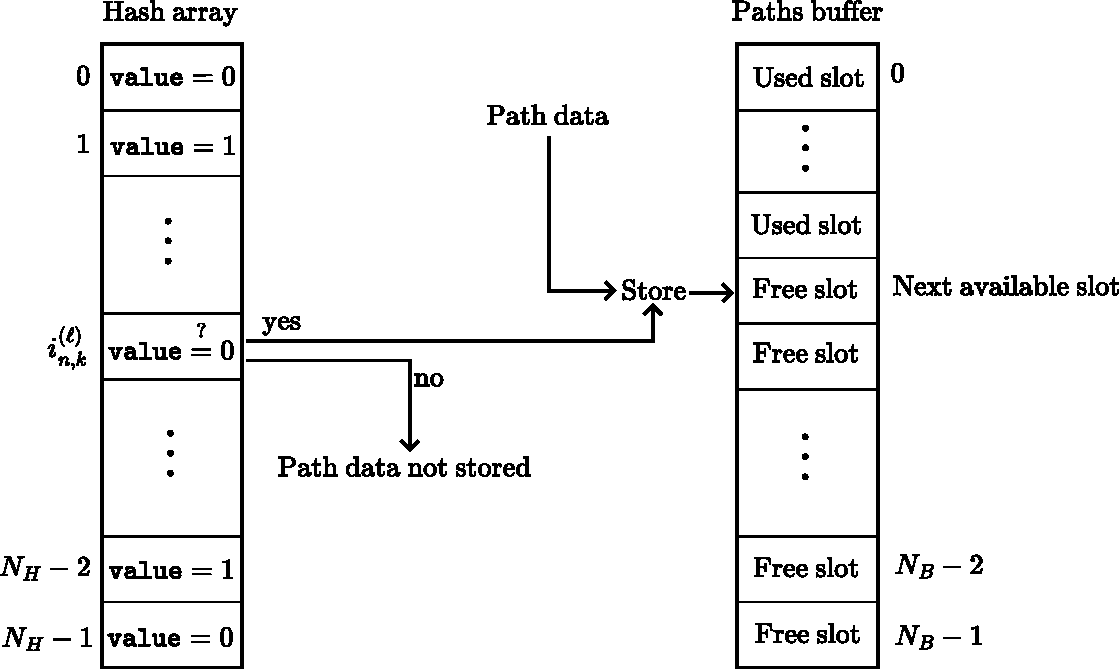
\includegraphics[width=0.8\textwidth]{figures/path-solver-hash-buffer.pdf}
    \caption{The hash array is used to track encountered path candidates. New candidates are stored in the buffer if they haven't been encountered before. Non-specular chains are added to the buffer without a uniqueness check (not depicted in the figure).\label{fig:path-solver-hash-buffer}}
\end{figure}

Valid paths and candidates are stored in a buffer of size $N_B$. This buffer holds, for each path, the sequence of interaction types, vertices, intersected objects, primitives, and more. When a valid path is found or a candidate is identified as unique, indicated by its corresponding entry $i_{n,k}^{(\ell)}$~\eqref{eq:path-solver-hash-mod} in the hash array being set to zero, the path data are stored in the buffer. It is important to note that the index $i_{n,k}^{(\ell)}$ is solely used for indexing the hash array and not for storing path data in the buffer. Instead, path data are stored contiguously in the next available slot of the path buffer, as shown in Figure~\ref{fig:path-solver-hash-buffer}. If the buffer becomes full, any newly found paths or candidates are discarded.
Discarding paths rather than overwriting existing ones is based on the reason that paths with lower depth, which are added to the buffer first as the \gls{SBR} loop advances from $\ell = 0$ to $\ell = L$, typically carry more energy and should not be replaced by higher depth paths when the buffer becomes full.
Consequently, the buffer size $N_B$ determines the maximum number of paths and candidates that can be stored.

Due to the substantial amount of data stored for each path, setting $N_B$ to excessively high values can lead to memory issues. This necessitates separating the hash array size $N_H$ from the buffer size $N_B$. This is because a small hash array size can increase the probability of collisions. To reduce the risk of collisions, $N_H$ is set to
\begin{equation}
    N_H = \max\LB N_B, 10^6 \RB
\end{equation}
ensuring a minimum array size of $10^6$ elements. In the interface of the \SRT{} built-in path solver, $N_B$ corresponds to the $\texttt{samples\_per\_src}$ parameter, and $N_H$ corresponds to $\texttt{max\_num\_paths\_per\_src}$.

\paragraph{Practical Consideration: Quantization Function}
An important practical consideration is the design of the quantization function $\texttt{Q}(\cdot)$.
When quantizing floating-point values to integers, values that are very close but lie on opposite sides of a quantization boundary can be mapped to different integers and therefore yield different hash values. For example, with rounding as the quantization function, $\texttt{Q}(1.4999)=1$ and $\texttt{Q}(1.5001)=2$.
This can cause identical candidates, which differ only due to numerical imprecision, to be treated as distinct, resulting in duplicate paths.
To mitigate this issue, multiple hash values are computed for each sample, each using a different quantization function. A path is only considered unique if all of its corresponding hash values are unique.
In the current implementation of \SRT{}, two quantization functions are used: rounding and floor, leading to two hash values being computed per candidate.
This approach can be interpreted as a form of locality-sensitive hashing~\cite{Wikipedia_Locality_Sensitive_Hashing}, as it aims to group together candidates that differ only due to numerical imprecision by using multiple hash functions to reduce the risk of misclassification.

\subsection{Image Method-based Candidate Processing}
\label{sec:path-solver-im}

The image method processes path candidates to determine valid paths that are specular chains, or end with specular suffixes. Consider a candidate path
\begin{equation}
    c_n^{(\ell)} = \left(\sv, \left(o_n^{(1)}, m_n^{(1)}, \iota_n^{(1)}, \chi_n^{(1)}\right), \cdots,  \underbrace{\left(o_n^{(\ell_d+1)}, m_n^{(\ell_d+1)}, \iota_n^{(\ell_d+1)}, \chi_n^{(\ell_d+1)}\right), \cdots, \left(o_n^{(\ell)}, m_n^{(\ell)}, \iota_n^{(\ell)}, \chi_n^{(\ell)}\right), \tv}_{\text{Specular suffix}}\right)
\end{equation}
where $\ell$ denotes the path depth, $\ell_d$ is the specular suffix index defined as in~\eqref{eq:essential-concepts-ell_d}, and $\tv$ is the target of the path.
Recall that the sequence of interactions $\boldsymbol{\chi}^{(\ell)} = \LB \chi_n^{(1)}, \cdots, \chi_n^{(\ell)} \RB$ was determined by the \gls{SBR}-based candidate generator.
For path candidates that end with a specular suffix but are not specular chains (i.e. $\ell_d > 0$), the image method processes only the specular suffix. In these cases, the vertex of the last diffuse reflection $\vv_n^{(\ell_d)}$ serves as the source point for the image method calculations.
Since the processing algorithm is identical for both specular chains and specular suffixes, we treat them equivalently in the following discussion. For simplicity of notation, we will refer to both types as specular chains and assume $\ell_d = 0$ throughout the remainder of this section.

\begin{figure}[htbp]
    \centering
    % First subfigure
    \begin{subfigure}[b]{0.45\textwidth}
        \centering
        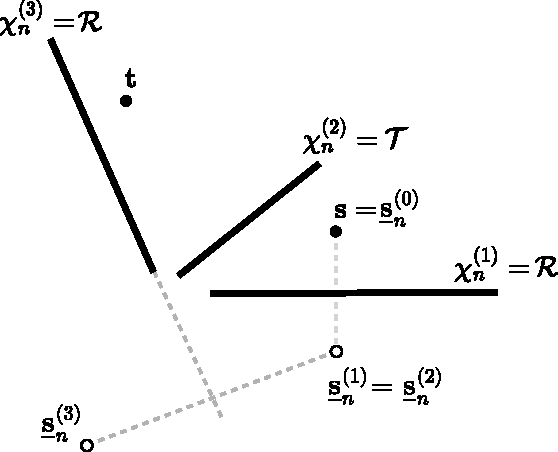
\includegraphics[width=0.8\textwidth]{figures/path-solver-im-step-1.pdf}
        \caption{\label{fig:path-solver-im-step-1}}
    \end{subfigure}
    \hfill
    % Second subfigure
    \begin{subfigure}[b]{0.45\textwidth}
        \centering
        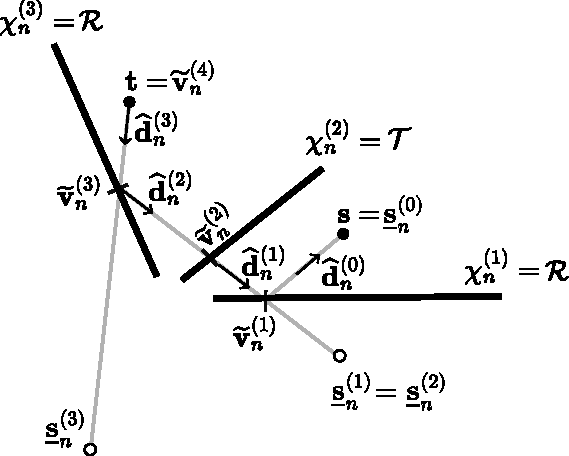
\includegraphics[width=0.8\textwidth]{figures/path-solver-im-step-2.pdf}
        \caption{\label{fig:path-solver-im-step-2}}
    \end{subfigure}
    \caption{The two steps of the image method for paths without diffraction: (a) compute the images of the source and (b) backtrack the path. Shown in 2D for clarity.\label{fig:path-solver-im}}
\end{figure}

\paragraph{Paths without Diffraction}
We begin by describing the image method process for candidates that contain no diffraction; as illustrated in Figure~\ref{fig:path-solver-im}, this process consists of two main steps. First, the method iteratively computes images of the source by reflecting it across each plane at which a specular reflection occurs.
Since refracted paths are modeled without angular deflection, incorporating refraction into the image method is straightforward: refractions may simply be skipped when computing the source images, as they do not alter the ray's direction.
Then, the algorithm backtracks from the target to determine the actual path vertices by intersecting lines between successive image sources.

Formally, the image method iteratively computes images of the source $\underline{\sv}_n^{(i)}$ for $i = 0, \dots, \ell$, starting from the original source $\sv$:
\begin{equation}
    \underline{\sv}_n^{(i)} = \begin{cases}
        \sv & \text{if } i = 0\\
        \underline{\sv}_n^{(i-1)} - 2\left( \left(\underline{\sv}_n^{(i-1)} - \pv_n^{(i)}\right)\tp \widehat{\nv}_n^{(i)}\right) \widehat{\nv}_n^{(i)}& \text{if } \chi_n^{(i)} = \Rc\\
        \underline{\sv}_n^{(i-1)} & \text{if } \chi_n^{(i)} = \Tc
    \end{cases}
\end{equation}
Here, $\pv_n^{(i)}$ represents any point on the plane containing the primitive $\LB o_n^{(i)}, m_n^{(i)} \RB$, and $\widehat{\nv}_n^{(i)}$ denotes the surface's normal vector. For specular reflections ($\chi_n^{(i)} = \Rc$), the image is computed by reflecting the previous image across the surface plane, while for refractions ($\chi_n^{(i)} = \Tc$), the image position remains unchanged.

During backtracking, the algorithm traces rays iteratively from the target $\tv$ back to the source $\sv$ by intersecting lines between successive image points.
The intersection points $\widetilde{\vv}_n^{(i)}$ are the refined vertices of the path.
Specifically, a sequence of $\ell$ rays $\LB \widetilde{\vv}_n^{(i+1)}, \widehat{\dv}_n^{(i)}\RB$, $i = \ell, \dots, 1$, is traced, where $\widetilde{\vv}_n^{(\ell+1)} = \tv$ and
\begin{equation}
    \label{eq:path-solver-im-backtracking}
    \begin{aligned}
        \widehat{\dv}_n^{(i)} &= \frac{\underline{\sv}_n^{(i)} - \widetilde{\vv}_n^{(i+1)}}{\norm{\underline{\sv}_n^{(i)} - \widetilde{\vv}_n^{(i+1)}}}\\
        \widetilde{\vv}_n^{(i)} &= \texttt{intersection}\left(\LB \widetilde{\vv}_n^{(i+1)}, \widehat{\dv}_n^{(i)} \RB, \LB o_n^{(i)}, m_n^{(i)} \RB\right), \text{only if } i > 0
    \end{aligned}
\end{equation}
where $\widetilde{\vv}_n^{(i)}$ is the intersection point between the ray $\LB \widetilde{\vv}_n^{(i+1)}, \widehat{\dv}_n^{(i)} \RB$ and the primitive $\LB o_n^{(i)}, m_n^{(i)} \RB$, as shown in Figure~\ref{fig:path-solver-im-step-2}.
The path is considered valid only if two conditions are met: (i) each ray $\LB \widetilde{\vv}_n^{(i+1)}, \widehat{\dv}_n^{(i)} \RB$ successfully intersects a primitive that is coplanar with the primitive $\LB o_n^{(i)}, m_n^{(i)} \RB$, and (ii) the line segment between $\widetilde{\vv}_n^{(i+1)}$ and $\widetilde{\vv}_n^{(i)}$ is unobstructed by any other scene geometry. If either condition fails, then the path is discarded.
The case $i = 0$ corresponds to the final segment of the path, which connects to the source $\sv$.
If the path is valid, then the returned path will be~\eqref{eq:path-solver-complete-cand}.

\paragraph{Paths with Diffraction}
To handle paths involving diffraction, we adopt an approach inspired by~\cite{6815738}. Since \SRT{} currently only supports first-order diffraction, each sample $n$ contains at most a single diffracting edge, whose position within the path is denoted by $i_{\Dc} \in \LP 1, \dots, \ell \RP$. For notational simplicity, we omit the explicit dependence of $i_{\Dc}$ on $n$.

The core idea is to use image theory to compute the diffraction point in image space and subsequently map it back to the original space.
The motivation for this approach is that, in the image space, all specular reflections and refractions are effectively ``removed'', leaving only the diffraction event.
This reduces the problem to a simpler form: finding the appropriate diffraction point for a path of the shape source $\rightarrow$ diffraction $\rightarrow$ target.
More precisely, for every sample $n$, the diffracting edge at depth $i_{\Dc}$, which is characterized by an endpoint $\ov_n$ and an edge vector $\widehat{\ev}_n$, has its images computed by reflecting its endpoint and edge vector across each plane at which a specular reflection occurs over the following interactions $i = i_{\Dc}+1, \dots, \ell$:
\begin{equation}
    \begin{aligned}
        \underline{\ov}_n^{(i)} &=
        \begin{cases}
            \ov_n & \text{if } i = i_{\Dc} \\
            \underline{\ov}_n^{(i-1)} & \text{if } \chi_n^{(i)} \neq \Rc \\
            \underline{\ov}_n^{(i-1)} - 2\left( \left(\underline{\ov}_n^{(i-1)} - \pv_n^{(i)}\right)\tp \widehat{\nv}_n^{(i)}\right) \widehat{\nv}_n^{(i)} & \text{if } \chi_n^{(i)} = \Rc
        \end{cases}\\
        \widehat{\underline{\ev}}_n^{(i)} &=
        \begin{cases}
            \widehat{\ev}_n & \text{if } i = i_{\Dc} \\
            \widehat{\underline{\ev}}_n^{(i-1)} & \text{if } \chi_n^{(i)} \neq \Rc \\
            \widehat{\underline{\ev}}_n^{(i-1)} - 2\left(\left(\widehat{\underline{\ev}}_n^{(i-1)}\right)\tp \cdot \widehat{\nv}_n^{(i)}\right) \widehat{\nv}_n^{(i)} & \text{if } \chi_n^{(i)} = \Rc
        \end{cases}
    \end{aligned}
\end{equation}
where $\pv_n^{(i)}$ represents any point on the plane containing the primitive $\LB o_n^{(i)}, m_n^{(i)} \RB$, and $\widehat{\nv}_n^{(i)}$ denotes the surface's normal vector.
Applying image theory, specular reflections and refractions can be ignored when searching for the diffraction point in image space.
The problem thus reduces to finding the diffraction point in image space, $\underline{\widetilde{\vv}}_n^{(i_{\Dc}, \ell)}$, of the path $\underline{\sv}_n^{(\ell)} \rightarrow \underline{\widetilde{\vv}}_n^{(i_{\Dc}, \ell)} \rightarrow \tv$.
According to Fermat's principle, the diffraction point minimizes the total path length, denoted by $\Lc(x_n)$.
Specifically,
\begin{align}
    \Lc(x_n) &=
        \norm{\tv - \underline{\widetilde{\vv}}_n^{(i_{\Dc}, \ell)}}
        +
        \norm{\underline{\sv}_n^{(\ell)} - \underline{\widetilde{\vv}}_n^{(i_{\Dc}, \ell)}} \label{eq:path-solver-diffraction-image-problem}
        \\
    \underline{\widetilde{\vv}}_n^{(i_{\Dc}, \ell)} &= \underline{\ov}_n^{(\ell)} + x_n \widehat{\underline{\ev}}_n^{(\ell)}
\end{align}
where $x_n \in \RR$.
For first-order diffraction, this minimization has a closed-form solution (see Annex~\ref{sec:diffraction-first-order}).

\begin{figure}[htbp]
    \centering
    \begin{subfigure}[b]{0.40\textwidth}
        \centering
        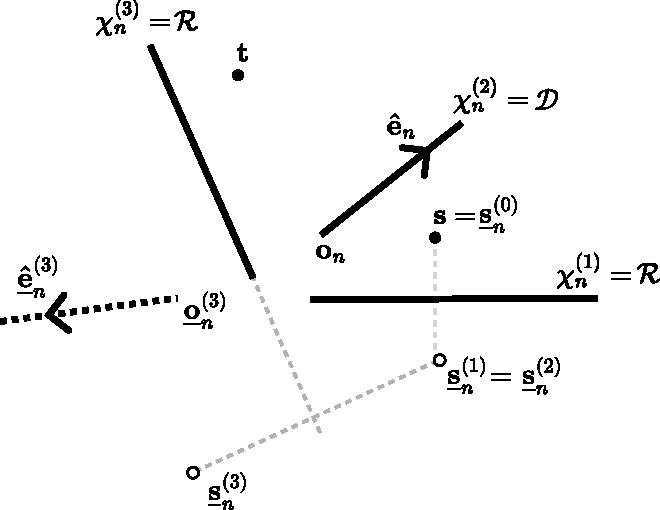
\includegraphics[width=\textwidth]{figures/path-solver-im-diffraction-step-1.pdf}
        \caption{\label{fig:path-solver-im-diffraction-step-1}}
    \end{subfigure}
    \hfill
    \begin{subfigure}[b]{0.18\textwidth}
        \centering
        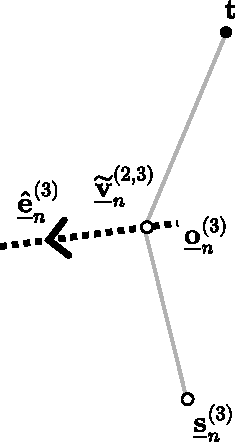
\includegraphics[width=0.75\textwidth]{figures/path-solver-im-diffraction-step-2.pdf}
        \caption{\label{fig:path-solver-im-diffraction-step-2}}
    \end{subfigure}
    \hfill
    \begin{subfigure}[b]{0.40\textwidth}
        \centering
        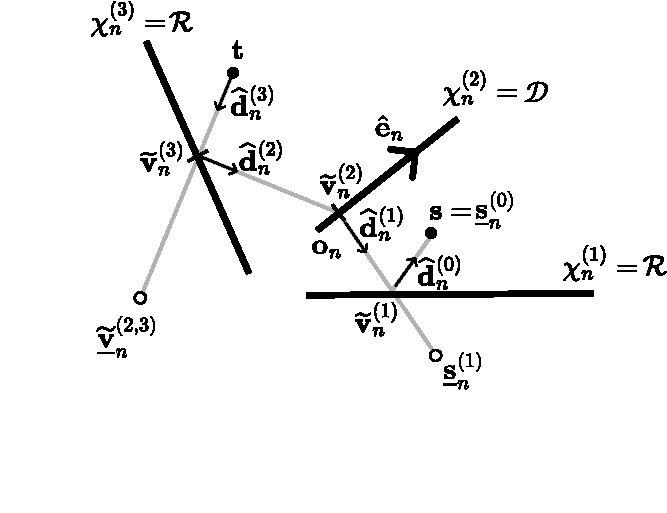
\includegraphics[width=\textwidth]{figures/path-solver-im-diffraction-step-3.pdf}
        \caption{\label{fig:path-solver-im-diffraction-step-3}}
    \end{subfigure}
    \caption{The three steps of the image method for paths with diffraction: (a) compute the images of the source, (b) compute the diffraction point in image space, and (c) backtrack the path. Shown in 2D for clarity.\label{fig:path-solver-im-step-diffraction}}
\end{figure}

Once the diffraction point is found in the image space, the refined path vertices $\widetilde{\vv}_n^{(i)}$, $i = 1, \dots, \ell$, are determined by backtracking as in the case without diffraction. However, for depths $i = i_{\Dc} + 1, \dots, \ell$, the algorithm uses the intermediate images of the diffraction point:
\begin{equation}
    \widetilde{\underline{\vv}}_n^{(i_{\Dc}, i)} = \underline{\ov}_n^{(i)} + x_n \widehat{\underline{\ev}}_n^{(i)}
\end{equation}
in place of $\underline{\sv}_n^{(i)}$ in~\eqref{eq:path-solver-im-backtracking}.
For $i = 1, \dots, i_{\Dc} - 1$, $\underline{\sv}_n^{(i)}$ is used as in the non-diffraction case.
The diffraction point is simply $\widetilde{\vv}_n^{(i_{\Dc})} = \ov_n + x_n \widehat{\ev}_n$.
This process is depicted in Figure~\ref{fig:path-solver-im-step-diffraction}.

\begin{figure}[ht!]
    \centering
    \begin{subfigure}[b]{0.45\textwidth}
        \centering
        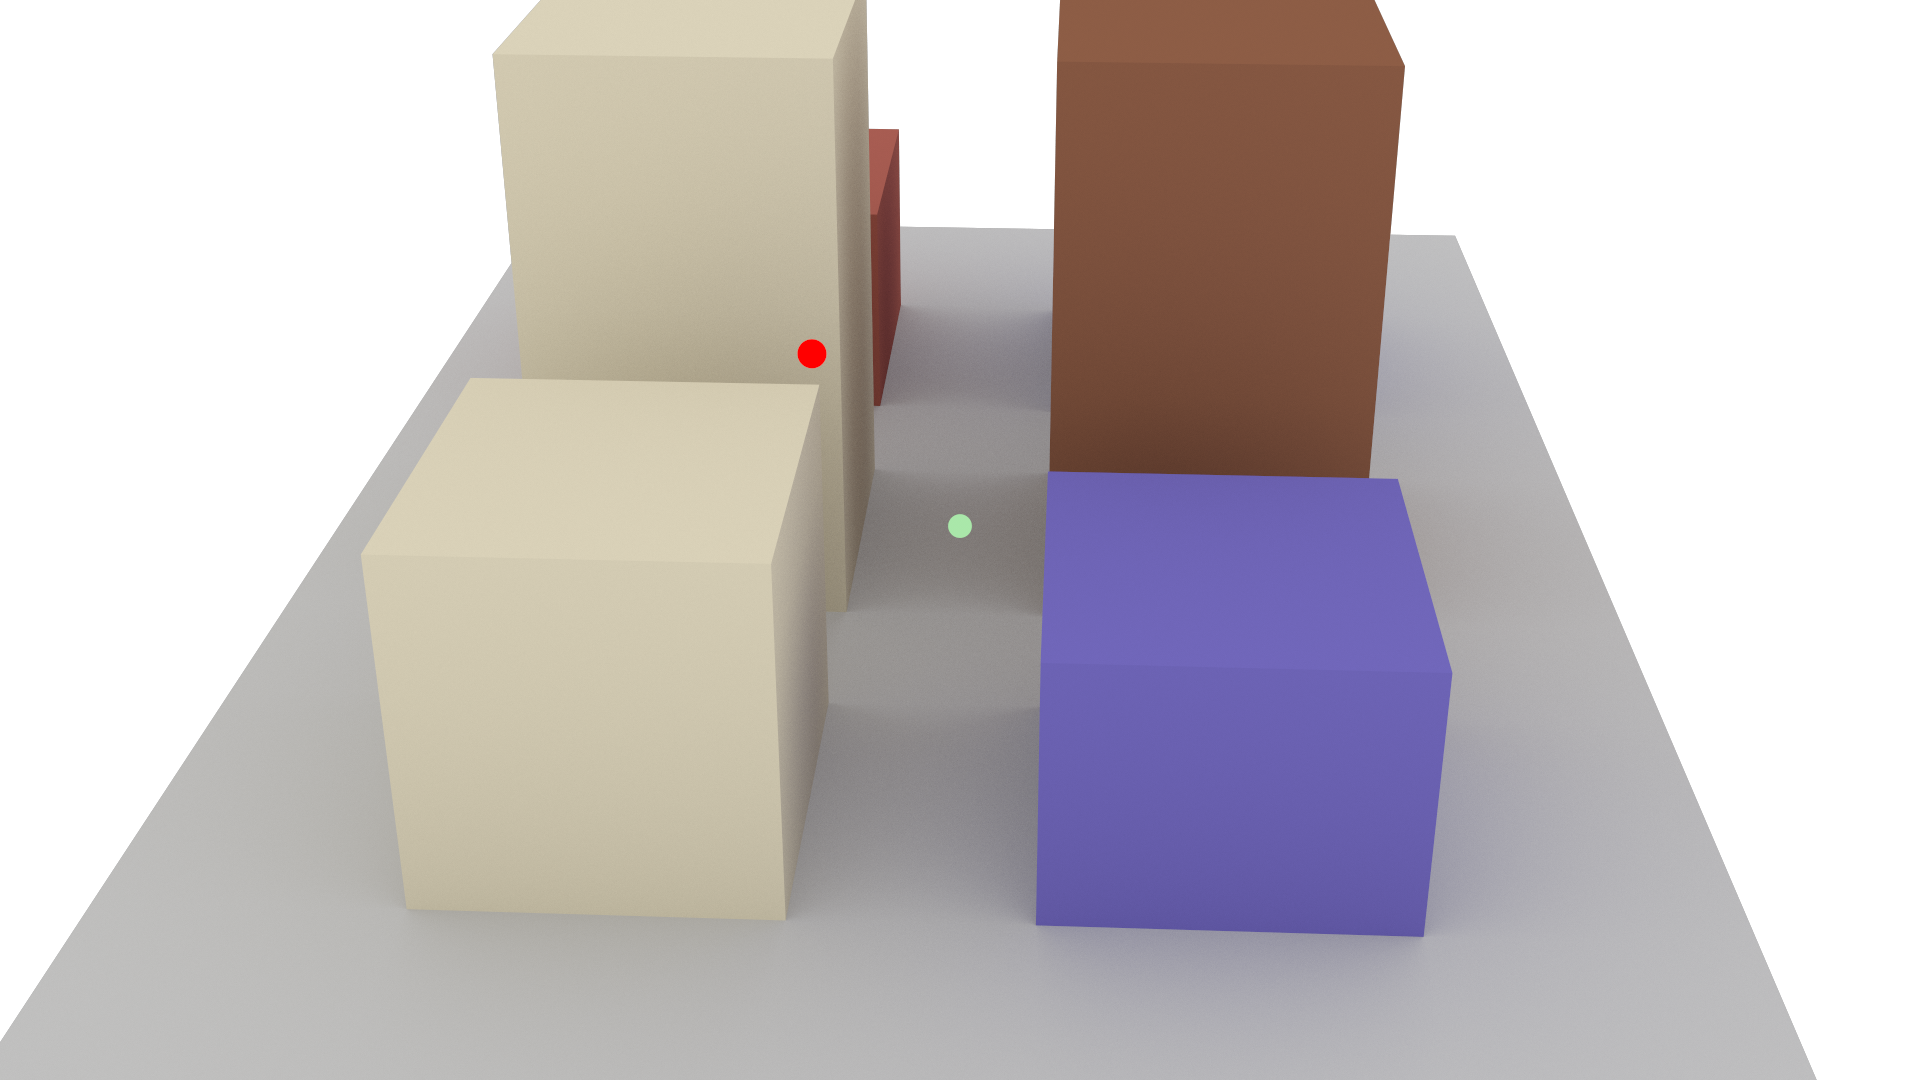
\includegraphics[width=\textwidth]{figures/simple-street-canyon-cam-2.png}
        \caption{Scene for this experiment. Red ball: source, green ball: target.\label{fig:path-solver-im-scene}}
    \end{subfigure}
    \hfill
    \begin{subfigure}[b]{0.45\textwidth}
        \centering
        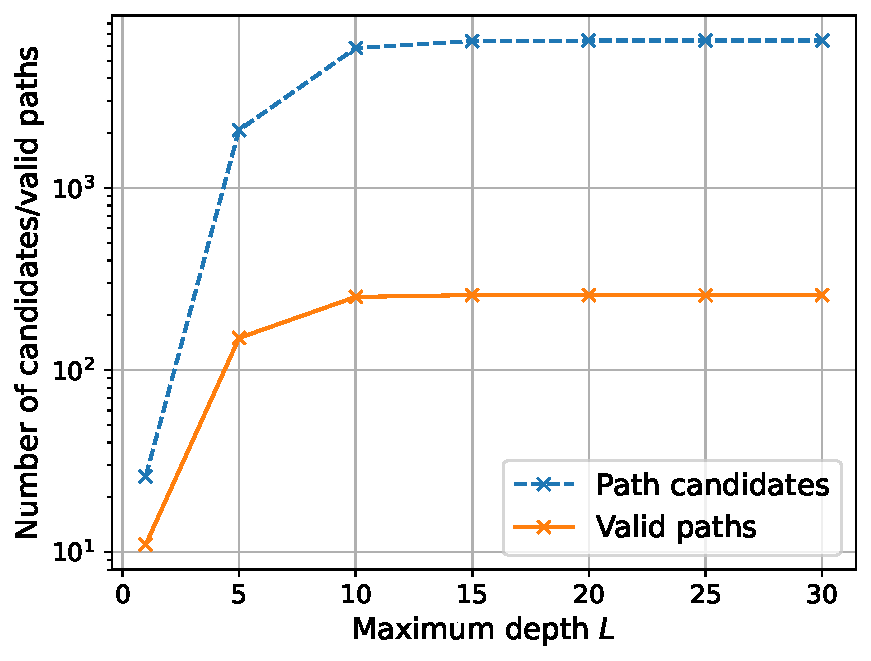
\includegraphics[width=\textwidth]{figures/path-solver-sbr-im.pdf}
        \caption{Number of candidates and valid paths.\label{fig:path-solver-gen-valid}}
    \end{subfigure}
    \caption{The image method typically discards most candidates.\label{fig:path-solver-sbr-im}}
\end{figure}

Typically, most of the candidates are discarded by the image method. This is illustrated in Figure~\ref{fig:path-solver-sbr-im}, which shows the number of candidates discarded as a function of the path depth for a single source and target. The considered scene is shown in Figure~\ref{fig:path-solver-im-scene}. The number of samples $N_S$ is $10^6$, diffuse reflection is disabled, and diffraction is enabled.
As seen in Figure~\ref{fig:path-solver-gen-valid}, most of the candidates are discarded by the image method because only specular chains are generated by the candidate generator, and most of them do not result in valid paths.

\subsection{Channel Coefficients, Delays, and Doppler Shifts Computation}
\label{sec:path-solver-em}

The final step of the path solver computes complex-valued channel coefficients and real-valued delays for each valid path (see Figure~\ref{fig:path-solver-archi}).
For clarity, we will focus our discussion on a single valid path with index $n$ and depth $\ell$, though the same procedure applies to all valid paths computed by both the \gls{SBR}-based candidate generator and image method.
We denote the path vertices as $\vv_n^{(i)},~i = 1, \dots, \ell$, which may correspond to vertices previously computed by the image method (denoted earlier as $\widetilde{\vv}_n^{(i)}$).
The directions of propagation between vertices are represented by unit vectors $\widehat{\kv}_n^{(i)},~i = 0, \dots, \ell$, defined as
\begin{equation}
    \widehat{\kv}_n^{(i)} = \frac{\vv_n^{(i+1)} - \vv_n^{(i)}}{\norm{\vv_n^{(i+1)} - \vv_n^{(i)}}},\qquad i = 0, \dots, \ell
\end{equation}
where $\vv_n^{(0)} = \sv$ is the source and $\vv_n^{(\ell+1)} = \tv$ is the target. Note that these propagation directions may differ from those used during the initial \gls{SBR} loop described in Section~\ref{sec:path-solver-sbr} due to the refinement by the image method.

\begin{figure}[ht!]
    \centering
    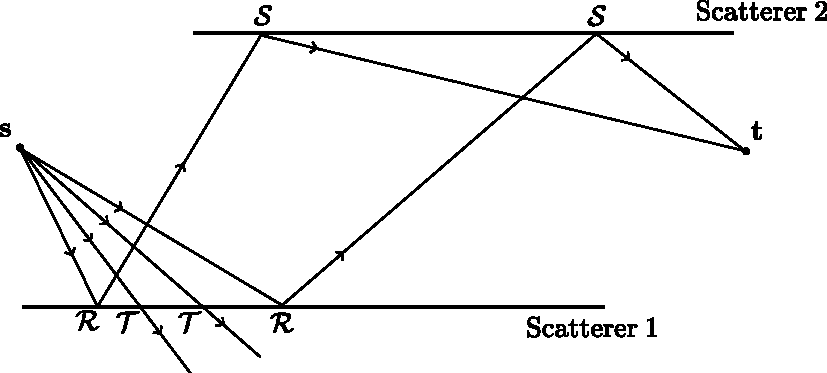
\includegraphics[width=0.6\textwidth]{figures/path-solver-energy.pdf}
    \caption{Due to the random sampling of interaction types, only some of the ray tubes that should reach the diffusely reflective surface (Scatterer 2) are traced. In this example, two out of four initial rays are transmitted when interacting with Scatterer 1, while the other two are reflected and reach the diffusely reflective surface.\label{fig:path-solver-energy}}
\end{figure}

\paragraph{Ensuring Energy Conservation}
As explained in Section~\ref{sec:path-solver-interaction-sampling}, at each interaction point, an interaction type is randomly chosen based on the probability distribution $\Qc$~\eqref{eq:path-solver-int-dist}. Initially, the energy emitted by the source is distributed across $N_S$ samples according to the transmit antenna pattern (see Section~\ref{sec:primer-em-tx-far-field}). Since only one interaction type is selected at each interaction point, ray tubes that do not match the chosen interaction type are discarded, as illustrated in Figure~\ref{fig:path-solver-energy}. The remaining ray tubes must therefore compensate for the discarded ones to maintain energy conservation. Given that there is a finite number of specular chains with a specific depth, the channel gain~\eqref{eq:channel-gain} observed at the target due to specular chains is accurate if all specular chains are identified by the path solver, which is assumed to be the case. This assumption will be reasonable if the number of samples $N_S$ is sufficiently large.

In the context of diffuse reflections, an incident ray tube scatters an amount of energy that is determined by its footprint on the diffusely reflective surface (see Section~\ref{sec:primer-em-diffuse}). Due to the random sampling of interaction types, only a portion of the ray tubes that should reach a diffusely reflective surface are actually traced (see Figure~\ref{fig:path-solver-energy}), which requires compensating for the untraced ones. For a given path $p^{(\ell)}$ that includes a diffuse reflection and has a specular suffix index $\ell_d$~\eqref{eq:essential-concepts-ell_d}, we denote by $\Pr \LB \boldsymbol{\chi}_n^{(\ell_d)} \RB = \prod_{\ell'=1}^{\ell_d} q \LB \chi_n^{(\ell')}\RB$ the probability of sampling the prefix leading to the last diffuse reflection point, where $q\LB \cdot \RB$ is defined in~\eqref{eq:path-solver-int-dist}. Consequently, on average, only a fraction $\Pr \LB \boldsymbol{\chi}_n^{(\ell_d)} \RB$ of the ray tubes that should reach the diffusely reflective surface are actually traced. To account for this, the electric field is scaled by $\nicefrac{1}{\sqrt{\Pr \LB \boldsymbol{\chi}_n^{(\ell_d)} \RB}}$ at the point of diffuse reflection.

\begin{algorithm}[ht!]
\caption{Electric field computation\label{alg:path-solver-electric-field}}
\begin{algorithmic}[1]
\State $\Em_n \gets \Call{tx\_pattern}{\widehat{\kv}^{(0)}_n}$ \Comment{Electric field vector}
\State $\tau_n \gets 0$ \Comment{Cumulative delay}
\State $r_n \gets 0$ \Comment{Length of the ray tube}
\State $\gamma_n \gets 1$ \Comment{Cumulative path probability}
\State $s_n \gets 0$ \Comment{Length of the incident ray tube on the diffracting edge}
\For{$\ell' = 1, \dots, \ell$}
    \State $\Tm_n^{(\ell')} \gets \Call{Evaluate\_Material}{o_n^{(\ell')}, \chi_n^{(\ell')}, \dots}$
    \State $\Em_n \gets \Tm_n^{(\ell')} \Em_n$
    \State $\gamma_n \gets \gamma_n \cdot q\LB \chi_n^{(\ell')}\RB$
    \State $r_n \gets r_n + \norm{\vv_n^{(\ell')} - \vv_n^{(\ell'-1)}}$
    \If{$\chi_n^{(\ell')} = \Sc$}
        \State $\Em_n \gets \frac{\Em_n}{\sqrt{\gamma_n}}$
        \State $\gamma_n \gets 1$
        \State $r_n \gets 0$
    \ElsIf{$\chi_n^{(\ell')} = \Dc$}
        \State $s_n \gets r_n$
        \State $r_n \gets 0$
    \EndIf
    \State $\tau_n \gets \tau_n + \frac{\norm{\vv_n^{(\ell')} - \vv_n^{(\ell'-1)}}}{c}$
\EndFor
\State $r_n \gets r_n + \norm{\tv - \vv_n^{(\ell)}}$
\State $\tau_n \gets \tau_n + \frac{\norm{\tv - \vv_n^{(\ell)}}}{c}$
\State $\Em_n^{\text{rx}} \gets \Call{rx\_pattern}{-\widehat{\kv}_n^{(\ell)}}$
\State $a_n \gets \frac{\lambda}{4\pi} \LB \Em_n\tp \Em_n^{\text{rx}} \RB$
\If{Diffracted path} \label{line:sf-start}
    \State $a_n \gets  \frac{a_n}{\sqrt{s_nr_n(s_n + r_n)}}$
\Else
    \State $a_n \gets \frac{a_n}{r_n}$
\EndIf \label{line:sf-end}
\State \Return $a_n,~\tau_n$
\end{algorithmic}
\end{algorithm}

\paragraph{Path Coefficient and Delay Computation}
Algorithm~\ref{alg:path-solver-electric-field} outlines the computation of the electric field along a path, based on the \gls{EM} background in Appendix~\ref{sec:primer-em}.
The algorithm calculates the electric field vector for each path by iterating through its sequence of interactions.
Computation begins by initializing the electric field $\Em_n$ with the transmit antenna pattern, evaluated in the initial departure direction $\widehat{\kv}_n^{(0)}$.
For dual polarization, two independent electric field vectors are tracked per path.
The variable $\tau_n$ accumulates the total propagation delay, and $r_n$ tracks the ray tube length; both start at zero.
The cumulative path probability $\gamma_n$, used for energy normalization, is initialized to one (see previous paragraph) and updated at each interaction.
The variable $s_n$ is only used for diffracted paths. For these paths, it accumulates the length of the incident ray tube on the diffracting edge, which is required to compute the diffraction spreading factor, i.e., the field intensity decrease factor due to free space propagation (see Section~\ref{sec:primer-em-diffraction}).

At each interaction, the electric field is updated by the transfer matrix $\Tm_n^{(\ell')}$, which depends on the intersected object $o_n^{(\ell')}$, the interaction type $\chi_n^{(\ell')}$, and other parameters (omitted for brevity). The path probability $\gamma_n$ is multiplied by the current interaction probability $q\LB \chi_n^{(\ell')}\RB$.
For diffuse reflections, the electric field is divided by $\sqrt{\gamma_n}$ to ensure energy conservation and $\gamma_n$ and $r_n$ are reset to one and zero, respectively, as diffuse reflection spawns a new ray tube.
For diffractions, the length of the incident ray tube on the diffracting edge $r_n$ is stored in $s_n$ and $r_n$ is reset to zero.
Each segment’s travel time is added to $\tau_n$, with $c$ the speed of light.

After processing all interactions, the algorithm adds the final segment to the target to both $\tau_n$ and $r_n$.
The receive antenna pattern is then evaluated for the incoming direction, and the channel coefficient is computed following Section~\ref{sec:primer-em-freq-ir}.
Finally, the spreading factor (lines~\ref{line:sf-start}--\ref{line:sf-end}) is computed and applied to the channel coefficient depending on whether the path involves diffraction or not.

\paragraph{Remark}
The transfer matrices $\Tm_n^{(\ell')}$ and the electric field vectors $\Em_n$ are complex-valued, but are implemented using their real-valued representations defined as
\begin{equation}
    \begin{bmatrix}
        \Re \LB \Tm_n^{(\ell')} \RB & -\Im \LB \Tm_n^{(\ell')} \RB\\
        \Im \LB \Tm_n^{(\ell')} \RB & \Re \LB \Tm_n^{(\ell')} \RB
    \end{bmatrix}
\end{equation}
for matrices and
\begin{equation}
    \begin{bmatrix}
        \Re\LB \Em_n \RB\\
        \Im\LB \Em_n \RB
    \end{bmatrix}
\end{equation}
for vectors, where $\Re{\LB \cdot \RB}$ and $\Im{\LB \cdot \RB}$ denote the real and imaginary parts, respectively.

\subsubsection{Handling Multiple Antennas at the Transmitter and Receiver}
\label{sec:path-solver-antenna-arrays}

As explained in the introduction (Section~\ref{sec:introduction}), \SRT{} supports antenna arrays of any size at both the transmitter and receiver, utilizing either synthetic or non-synthetic arrays. In the case of non-synthetic arrays, each transmit antenna is treated as a source and each receive antenna as a target, meaning paths are traced from every transmit antenna, and the solver calculates paths for each transmit-receive antenna pair. For synthetic arrays, paths originate from a single ``virtual'' source at the center of the transmitter array, and a single ``virtual'' target is considered at the center of every receiver array. Channel coefficients are then computed by applying phase shifts synthetically. This method allows for efficient scaling with the number of antennas, but it is an approximation that is valid only when the transmitter and receiver array sizes are small relative to the distance from the radio devices to each other and to the scatterers. Formally, for synthetic arrays, the channel matrix for the $n$-th path is expressed as:
\begin{equation}
    \Hm_{\text{array}, n} = a_n \uv_A^{\text{rx}} \LB \uv_A^{\text{tx}} \RB\tp
\end{equation}
where $a_n$ is the channel coefficient for the $n$-th path, calculated using Algorithm~\ref{alg:path-solver-electric-field}. The array response vectors for the transmit ($\uv_A^{\text{tx}}$) and receive ($\uv_A^{\text{rx}}$) antenna arrays are defined as:
\begin{equation}
    \label{eq:path-solver-array-response-vector}
    \begin{aligned}
        \uv_A^{\text{tx}} &= \LSB e^{j \frac{2\pi}{\lambda}\LB \widehat{\kv}_n^{(0)} \RB \tp\dv_1^{\text{tx}}}, \cdots, e^{j \frac{2\pi}{\lambda}\LB \widehat{\kv}_n^{(0)} \RB \tp\dv_{N_A^{\text{tx}}}^\text{tx}} \RSB\tp,\\
        \uv_A^{\text{rx}} &= \LSB e^{j \frac{2\pi}{\lambda}\LB -\widehat{\kv}_n^{(\ell)} \RB \tp\dv_1^{\text{rx}}}, \cdots, e^{j \frac{2\pi}{\lambda}\LB -\widehat{\kv}_n^{(\ell)} \RB \tp\dv_{N_A^{\text{rx}}}^\text{rx}} \RSB\tp.
    \end{aligned}
\end{equation}
Here, $\widehat{\kv}_n^{(0)}$ ($\widehat{\kv}_n^{(\ell)}$) represents the departure (arrival) direction of the $n$-th path, $N_A^{\text{tx}}$ ($N_A^{\text{rx}}$) denotes the number of antennas in the transmit (receive) array, and $\dv_i^{\text{tx}}$ ($\dv_i^{\text{rx}}$) indicates the relative position of the $i$-th antenna element to the virtual source (target) in the transmit (receive) array.

\subsubsection{Doppler Shifts}

The impact of moving scene objects on the paths can be simulated in two ways.
The first approach involves moving objects in small incremental steps along their trajectories and recomputing the propagation paths at each step.
While this method provides the highest accuracy, it is computationally expensive.
However, when trajectory lengths are small (not exceeding a few wavelengths), a more efficient approach may be used.
In this alternative method, we assign a velocity vector $\boldsymbol{\varv}\LB o \RB \in \RR^3$ to each object $o$ and compute the time evolution by accumulating Doppler shifts along the propagation paths.

\begin{figure}[t]
    \centering
    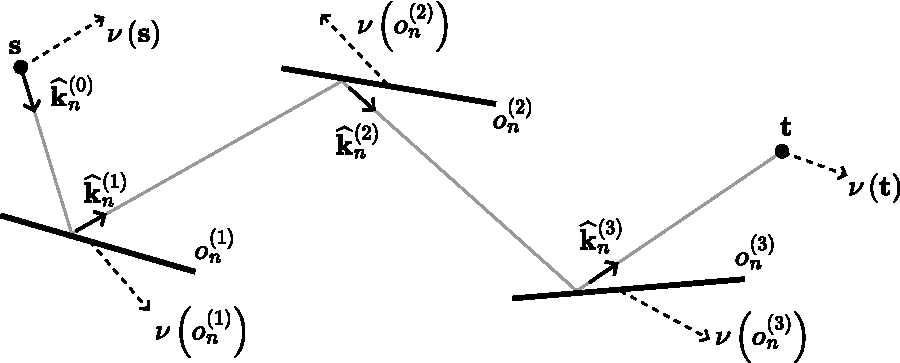
\includegraphics[width=0.6\textwidth]{figures/path-solver-doppler.pdf}
    \caption{Each object as well as the source and target has an associated velocity vector that contributes to the total Doppler shift. Shown in 2D for clarity.\label{fig:path-solver-doppler}}
\end{figure}

Figure~\ref{fig:path-solver-doppler} illustrates this approach.
When replaying the valid paths using Algorithm~\ref{alg:path-solver-electric-field}, the Doppler shift for each path $n$ is computed by accumulating the contributions from individual objects:
\begin{equation}
    \nu_n^{(\ell')} =
    \begin{cases}
        0 & \text{if } \ell' = 0\\
        \nu_n^{(\ell'-1)} + \frac{\boldsymbol{\varv}\LB o_n^{(\ell')} \RB\tp \LB \widehat{\kv}_n^{(\ell')} - \widehat{\kv}_n^{(\ell'-1)} \RB}{\lambda} & \text{if } 1 \leq \ell' < \ell\\
    \end{cases}
\end{equation}
where $\lambda$ is the wavelength. This results in the total Doppler shift $\nu_n^{(\ell)}$ caused by object movements along the path. The final Doppler shift observed at the target combines the accumulated shift from moving objects with the shifts caused by source and target motion:
\begin{equation}
    \nu_n = \nu_n^{(\ell)} + \frac{\boldsymbol{\varv}\LB \sv \RB\tp \widehat{\kv}_n^{(0)}}{\lambda} - \frac{\boldsymbol{\varv}\LB \tv \RB\tp \widehat{\kv}_n^{(\ell)}}{\lambda}.
\end{equation}
where $\boldsymbol{\varv}\LB \sv \RB \in \RR^3$ and $\boldsymbol{\varv}\LB \tv \RB \in \RR^3$ denote the velocity vectors of the source and target, respectively.

\subsection{Current Limitations and Potential Improvements}
\label{sec:path-solver-limitations}

We discuss in this section some current limitations and potential improvements of the path solver.

\paragraph{Sampling of Ray Directions}

\begin{figure}[ht!]
    \centering
    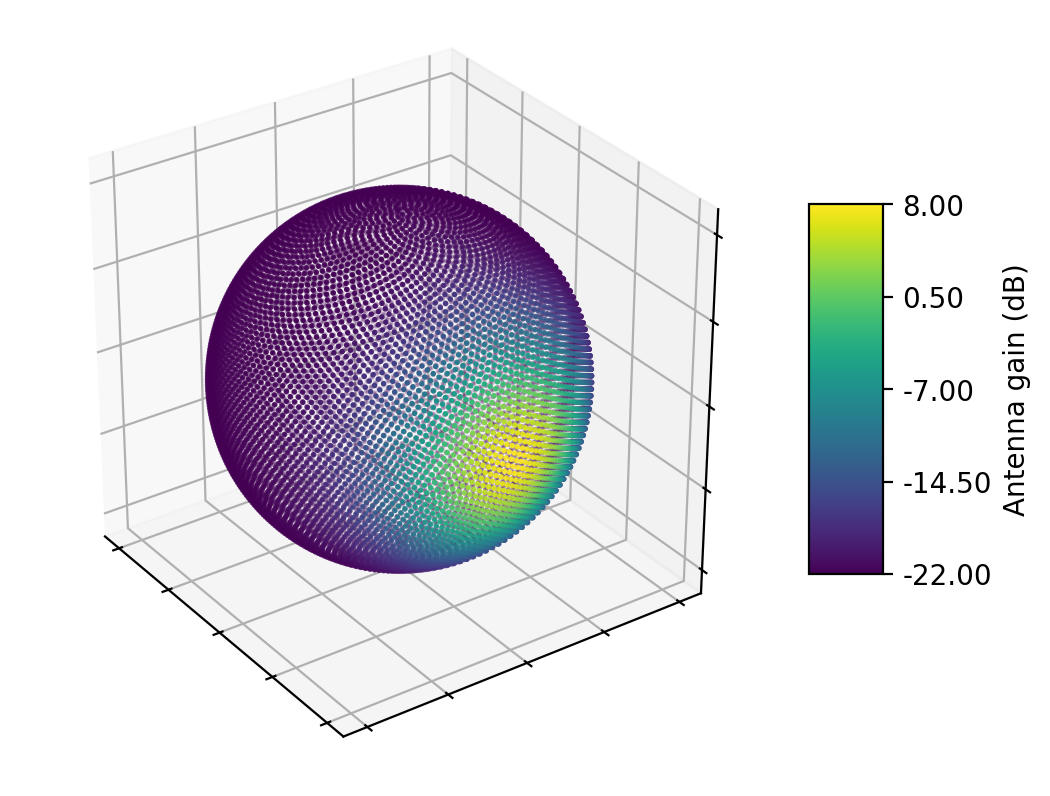
\includegraphics[width=0.55\textwidth]{figures/path-solver-is-ant-pattern.png}
    \caption{Gain of the 3GPP TR 38.901~\cite[Table~7.3-1]{TR38901} antenna pattern for each sample direction on a Fibonacci lattice with $10^4$ points. The majority of sample directions exhibit low gain, indicating that importance sampling of ray directions may be beneficial.\label{fig:path-solver-is-ant-pattern}}
\end{figure}

Improved sample efficiency could be achieved by sampling initial ray directions and scattered ray directions based on the transmit antenna pattern and the scattering pattern, respectively. This approach is motivated by the substantial sample efficiency gains shown in Section~\ref{sec:path-solver-interaction-sampling} through the use of importance sampling. By applying optimized sampling strategies for ray directions, further improvements may be realized, as illustrated in Figure~\ref{fig:path-solver-is-ant-pattern}.

\paragraph{Handling Large Numbers of Targets and Sources}

\begin{figure}[ht!]
    \centering
    \begin{subfigure}[b]{0.50\textwidth}
        \centering
        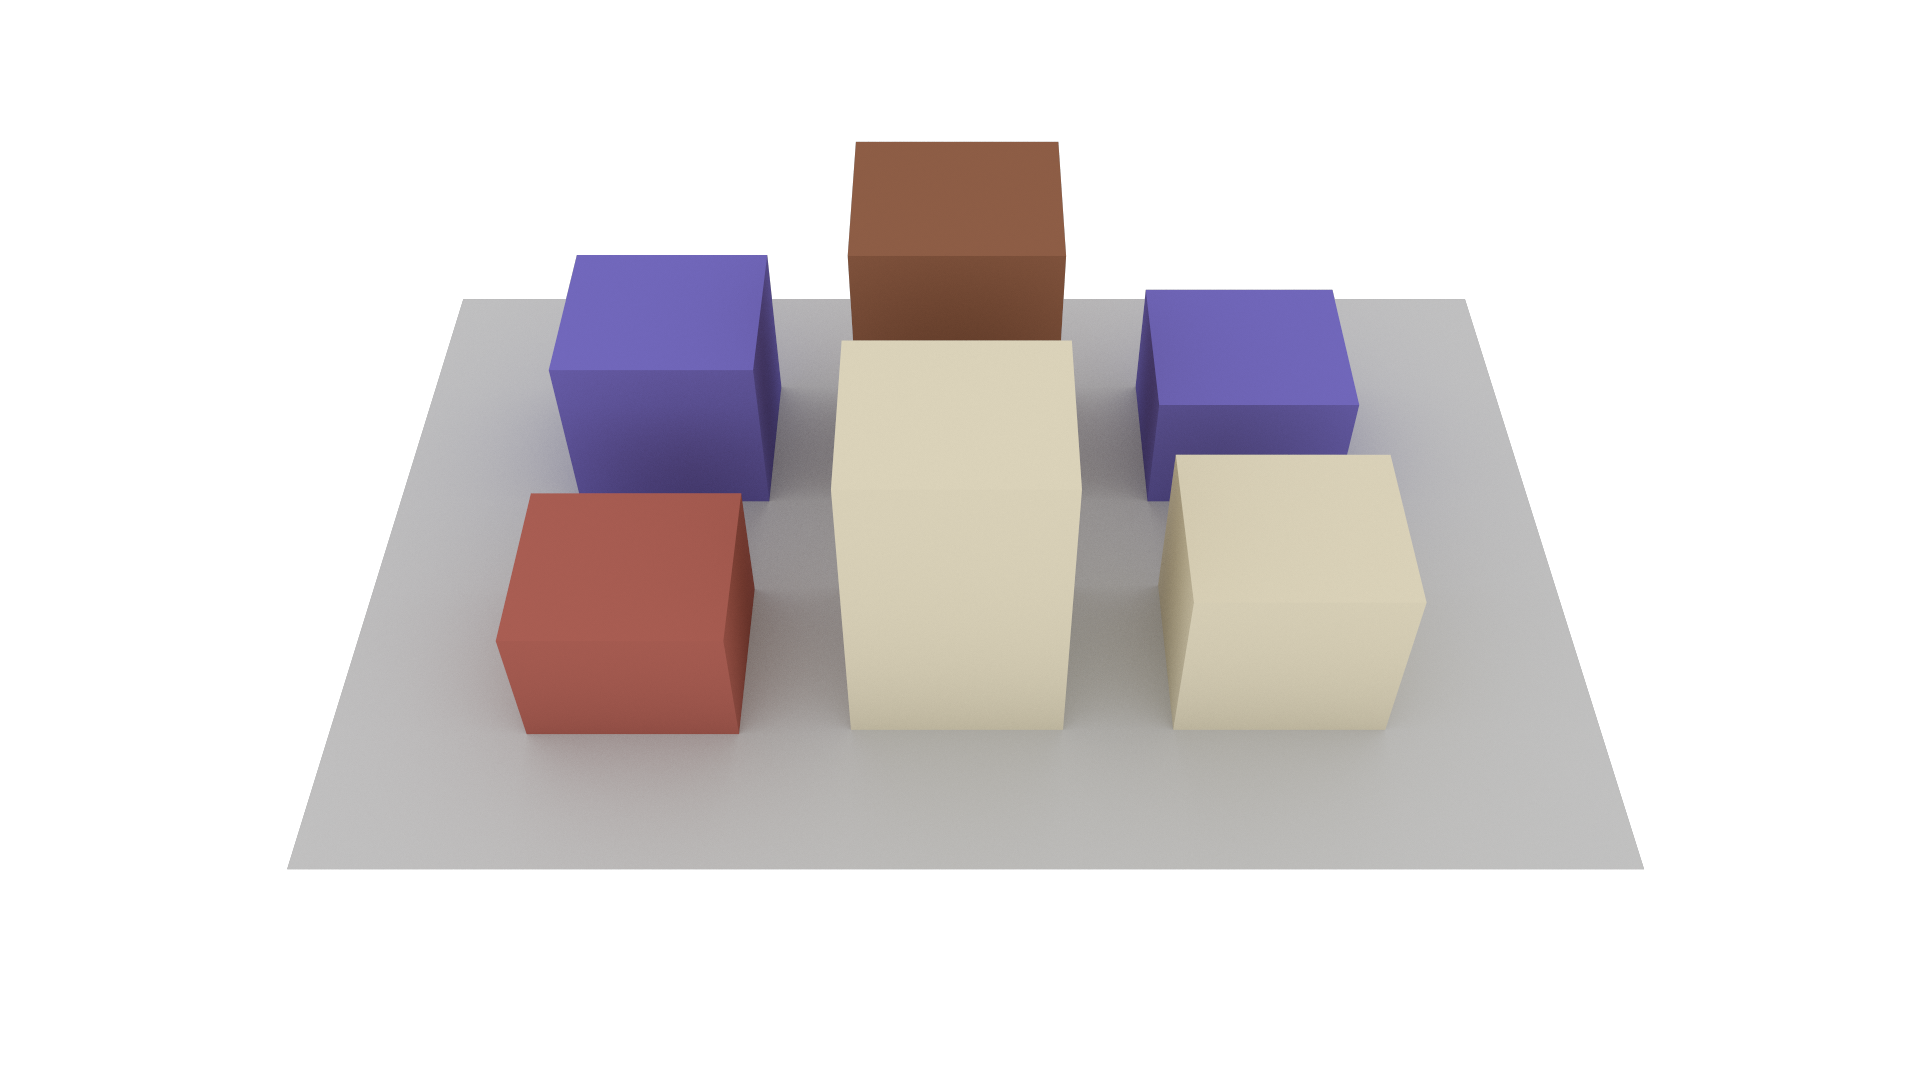
\includegraphics[width=\textwidth]{figures/simple-street-canyon-cam.png}
        \caption{Considered scene.\label{fig:simple-street-canyon}}
    \end{subfigure}
    \hfill
    \begin{subfigure}[b]{0.49\textwidth}
        \centering
        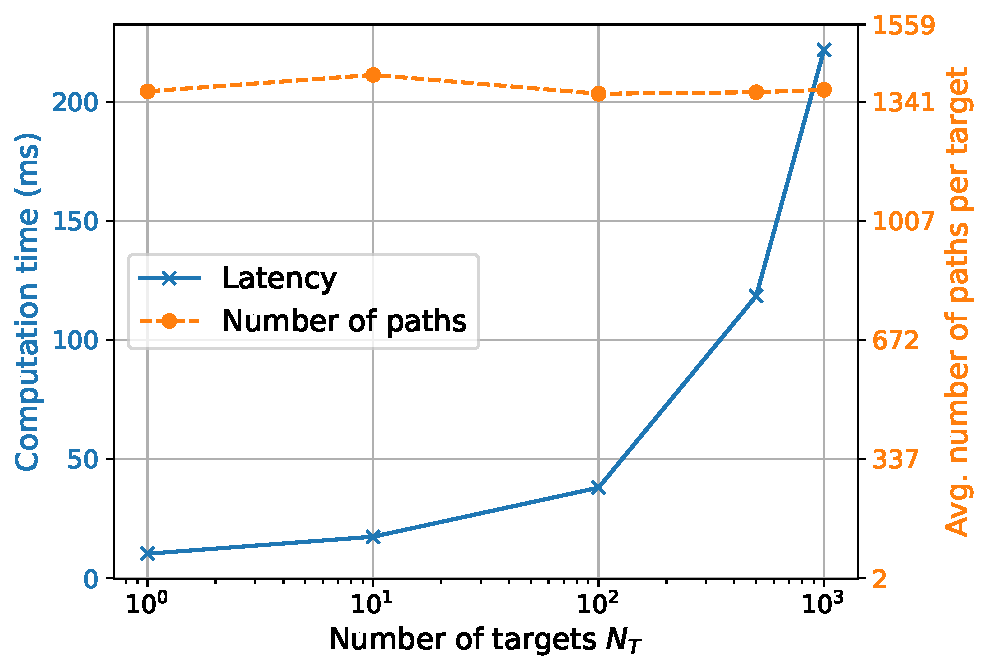
\includegraphics[width=\textwidth]{figures/path-solver-sbr-tgt.pdf}
        \caption{Compute time and number of candidates found vs. the number of targets.\label{fig:path-solver-sbr-tgt}}
    \end{subfigure}

    \begin{subfigure}[b]{0.49\textwidth}
        \centering
        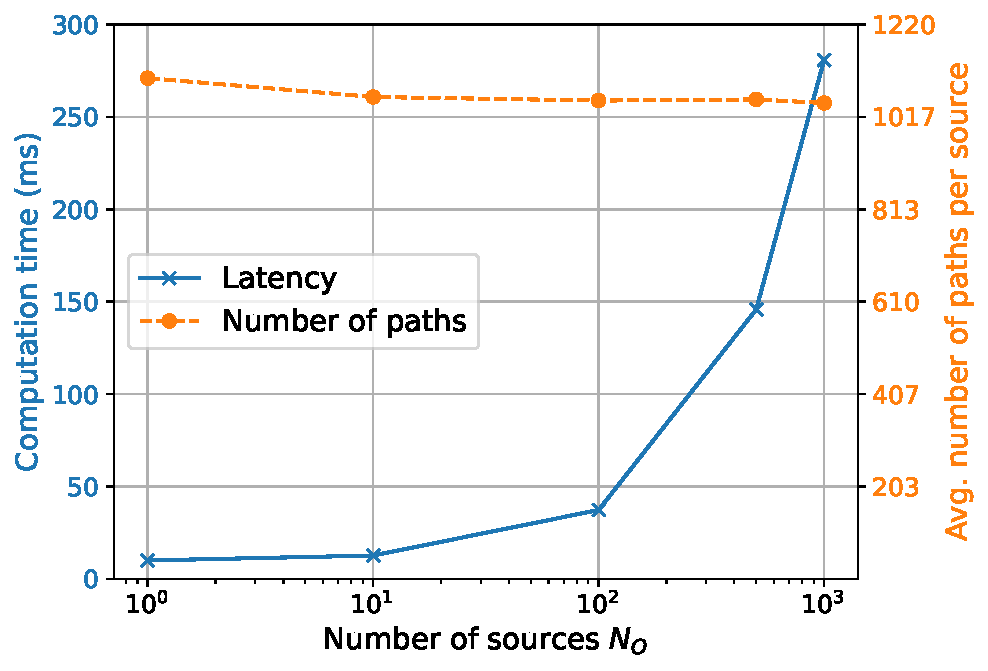
\includegraphics[width=\textwidth]{figures/path-solver-sbr-src-cst-samples-per-src.pdf}
        \caption{Compute time and number of candidates found vs. the number of sources and with a constant number of samples per source.\label{fig:path-solver-sbr-src-cst-samples-per-src}}
    \end{subfigure}
    \hfill
    \begin{subfigure}[b]{0.49\textwidth}
        \centering
        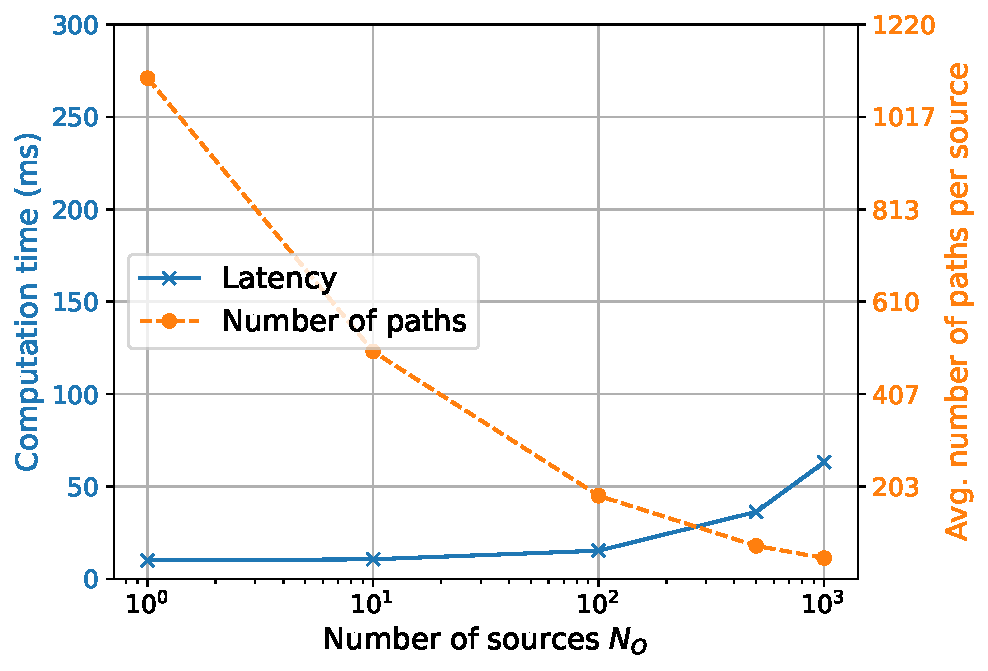
\includegraphics[width=\textwidth]{figures/path-solver-sbr-src-cst-total-samples.pdf}
        \caption{Compute time and number of candidates found vs. the total number of samples with a constant number of samples in total.\label{fig:path-solver-sbr-src-cst-total-samples}}
    \end{subfigure}
    \caption{Computation time and number of candidates found as a function of the number of sources and targets. The experiments are conducted on an NVIDIA RTX 4090 GPU.\label{fig:path-solver-sbr-src-tgt}}
\end{figure}

The current method for handling multiple targets involves iterating over all targets during each \gls{SBR} loop iteration. Figure~\ref{fig:path-solver-sbr-tgt} illustrates this, showing the compute time of the candidate generator and the average number of candidates per target found as the number of targets varies. In this experiment, the built-in \SRT{} scene ``simple street canyon'' depicted in Figure~\ref{fig:simple-street-canyon}, was used. Targets were sampled uniformly at random on a plane parallel to the ground at an elevation of 1.5 meters. The maximum depth $L$ was set to 5, diffuse reflections were disabled, and the number of samples $N_S$ was set to $10^6$. As observed, the compute time increases with the number of targets due to the iteration over all targets in each \gls{SBR} loop iteration. However, the number of candidates per target remains stable, although with variations due to hash collisions. Note that, as discussed in Section~\ref{sec:path-solver-im}, most candidates do not result in valid paths.
This approach may be optimized by selecting only targets near intersection points or the source, which will enhance scalability when dealing with a large number of targets.

Scaling with the number of sources presents its own set of challenges. When $N_S$ samples are generated per source, the total number of samples produced by the candidate generator becomes $N_S \cdot N_O$, where $N_O$ denotes the number of sources. This results in increased computation time as the number of sources grows, as illustrated in Figure~\ref{fig:path-solver-sbr-src-cst-samples-per-src}. However, the number of candidates per source remains stable. In this experiment, a single target is positioned at the center of the scene at an elevation of 1.5 meters, while sources are randomly sampled on a plane parallel to the ground at an elevation of 70 meters, above all buildings. Recall that variations in the number of candidates per source may occur due to collisions. For a comprehensive view, Figure~\ref{fig:path-solver-sbr-src-cst-total-samples} presents results where the total number of samples is kept constant at $10^6$, resulting in $N_S = \left\lfloor \frac{10^6}{N_O} \right\rfloor$ samples per source. In this scenario, the computation time increases at a much slower rate with the number of sources, but the number of candidates found per source decreases rapidly as the number of sources increases.

\paragraph{Higher-Order Diffraction and Diffuse Reflection}

The path solver supports only first-order diffraction and does not handle paths that contain both diffraction and diffuse reflection. Enabling support for such combined paths would require the refinement of non-suffix path segments, which is computationally expensive and thus not implemented at present. However, these mixed paths typically transport a negligible amount of energy and therefore have little impact on the accuracy of the computed \glspl{CIR}.

Regarding high-order diffraction, there are algorithms for determining the diffraction vertices~\cite{4200889}. However, calculating the electric field along these high-order diffraction paths remains an open problem, and as a result, high-order diffraction is not currently supported.

\paragraph{Collisions of Specular Chain Candidates}

The path solver does not handle collisions of specular chain candidates.
More precisely, when two different specular chains share the same index value in the hash array despite having a different hash due to the modulo operation~\eqref{eq:path-solver-hash-mod}, the path solver discards one of them. This could be avoided by using a collision resolution mechanism, and by dynamically adjusting the hash array size to reduce the probability of collisions.
Currently, it is assumed that the hash array size is set to a sufficiently large value to make collisions negligible.
